%% Nature Computational Science submission --- Springer Nature template (sn-jnl).
%% Build: ./build.sh -> main.pdf and si.pdf. main.tex and si.tex cross-reference each other's labels through the
%% xr package, so each is compiled around the other's .aux (see build.sh); ./build.sh clean builds the same text
%% through the wrapper files main_clean.tex / si_clean.tex (main_clean.pdf / si_clean.pdf).
%% Display items (6): Fig 1 overview + attainment (a-p); Fig 2 regret trajectories (a-m); Fig 3 controlled-grid
%% final-regret advantage maps (a-c); Fig 4 calibration versus attainment (a-m); Fig 5 top-k overlap, LF-screening
%% regret and compute scaling (a-c); Table 1 benchmark suite. SI: Supplementary Notes 1-6, Figs 1-3, Tables 1-4.

\documentclass[pdflatex,sn-nature,iicol]{sn-jnl}% Nature Portfolio two-column journal layout

%============================================================================

%%%% Standard packages. Note: the sn-jnl class assumes xcolor / textcomp /
%%%% manyfoot are loaded (it uses them in its \begin{document} hook), so they
%%%% are kept here even though the original ICML preamble did not list them.
\usepackage{graphicx}%
\usepackage{amsmath,amssymb,amsfonts}%
\usepackage{mathtools}%
\usepackage{xcolor}%
\usepackage{textcomp}%
\usepackage{manyfoot}%
\usepackage{booktabs}%
\usepackage{array}%
\usepackage{microtype}%
\usepackage[title]{appendix}%

%% Tighten Springer Nature's default page margins (the class leaves a very
%% large bottom margin and ~24mm sides). This widens the two-column text block
%% and reduces whitespace while keeping the two-column journal layout.
\geometry{a4paper, top=16mm, bottom=18mm, left=18mm, right=18mm,
          marginparwidth=0mm, marginparsep=0mm, bindingoffset=0mm, columnsep=8mm}

\raggedbottom

%% Corresponding-author asterisk. sn-jnl.cls emits it inside
%%   \authorsep{#2}\unskip\ifx\@authfrstarg\empty\else ... {*} ... \fi
%% in \@@corrauthor, where \@authfrstarg is the OPTIONAL affiliation argument.
%% All four authors share one affiliation, so no affiliation superscripts are
%% wanted and \author* is written without brackets -- which skips that branch
%% entirely and leaves the "*Corresponding author(s)" footnote with no asterisk
%% anchored to any name. Redefine the macro to print the asterisk
%% unconditionally, and no affiliation number. (Delete this patch and restore
%% \author*[n] / \affil[n] if a second affiliation is ever added.)
\makeatletter
\renewcommand{\@@corrauthor}[2][]{\def\@authfrstarg{#1}\@corauemailtrue%
  \advance\corraucount by 1%
  \g@addto@macro\artauthors{%
    \global\@auemailtrue%
    \Authorfont%
    \def\baselinestretch{1}%
    \authorsep{#2}\unskip\textsuperscript{*}\unskip%
    \def\authorsep{\au@and~}%
    \global\let\sep\@empty\global\let\@corref\@empty%
  }}%
\makeatother

%% The Supplementary Information lives in si-content.tex. For submission, main.tex
%% and si.tex are built as separate PDFs and cross-reference each other's labels
%% through the xr package (build.sh). Define \withSI to build one combined PDF.
\ifdefined\withSI\else
\usepackage{xr}
%% Import only the labels of the other file: natbib's \bibcite entries in its .aux
%% must not override this document's own citation numbers.
\makeatletter\let\XR@savedbibcite\bibcite\let\bibcite\@gobbletwo
\externaldocument{si}
\let\bibcite\XR@savedbibcite\makeatother
\fi

\begin{document}

\title[Transfer Learning Architectures for Scalable Multi-Fidelity Bayesian
Optimization]{Transfer Learning Architectures for Scalable Multi-Fidelity Bayesian
Optimization}

\author{\fnm{Jaewook} \sur{Lee}}

\author{\fnm{Ethan} \sur{Errington}}

\author{\fnm{Christian D.} \sur{Lorenz}}

\author*{\fnm{Miao} \sur{Guo}}\email{miao.guo@kcl.ac.uk}

\affil{\orgdiv{Department of Engineering}, \orgname{King's College London},
\orgaddress{\city{London}, \postcode{WC2R 2LS}, \country{United Kingdom}}}
\abstract{\unboldmath Self-driving laboratories combine abundant low-fidelity evaluations with scarce high-fidelity experiments through multi-fidelity Bayesian optimization, where the surrogate model guides experimental decisions. Gaussian processes remain the standard surrogate but can become restrictive in complex molecular and materials spaces. Here we investigate how surrogate choice governs multi-fidelity optimization by evaluating five transfer-learning architectures and three Gaussian-process methods under matched budgets, fidelity schedules and initial designs across thirteen optimization tasks. We find that Gaussian processes perform best on the smooth, two-dimensional Branin functions, whereas on every chemistry and materials benchmark the best transfer-learning surrogate matches or exceeds the best Gaussian process in mean attainment. Separate compute profiles on nine tasks show up to 22-fold fewer floating-point operations for transfer-learning surrogates. A controlled 126-condition grid shows that this advantage tracks preservation of near-optimal candidate rankings more strongly than global low--high-fidelity correlation, while matched-acquisition experiments attribute it primarily to the surrogate. These results recast multi-fidelity optimization in complex scientific search spaces as a representation-learning problem.}

\keywords{Multi-fidelity Bayesian optimization, Transfer learning,
Materials and molecular discovery}

\maketitle

\section{Introduction}

Self-driving laboratories (SDLs) are transforming scientific discovery by integrating automated experimentation with AI-driven decision-making in closed-loop optimization workflows. In SDL systems, experiments are designed, executed and analysed autonomously, while the derived data iteratively update a surrogate model that guides subsequent experimentation\citep{abolhasani2023rise,
hickman2025atlas}. As the decision-making core of the SDL, the surrogate model and acquisition policy largely determine the efficiency of discovery. In chemistry and
materials science, where experimental search spaces are vast and evaluations are expensive, Bayesian
optimization (BO) has therefore become the dominant approach for identifying optimal conditions with fewer evaluations\citep{shahriari2015taking}.

A central limitation of conventional BO is its reliance on a single source of information, which imposes a trade-off between evaluation cost and prediction accuracy. Scientific and engineering problems naturally possess hierarchical sources of information spanning multiple fidelities \citep{peherstorfer2018survey}. Low-fidelity (LF) evaluations, such as approximate simulations or reduced-order models, are inexpensive but often noisy, biased or approximate. High-fidelity (HF) experiments and rigorous simulations provide substantially greater accuracy, but at far higher cost and lower throughput. Multi-fidelity Bayesian optimization (MFBO) addresses this challenge by combining these complementary information sources within a unified optimization framework, enabling  inexpensive LF evaluations to broadly explore the
design space while reserving scarce HF measurements for validation of the most promising
candidates~\citep{kennedy2000predicting}. MFBO has therefore emerged as an increasingly powerful strategy for
improving sample efficiency in autonomous discovery under constrained experimental budgets~\citep{sabanza2025best}.

\begin{figure*}[tp]
\centering
%% Display item 1 of 6: (a) overview (paper_figures/fig1_overview.tex; the letter is overlaid in LaTeX below) and
%% (b--p) attainment on the 13 benchmarks (fig1_attainment.pdf, letters baked in); overview at 0.9\textwidth so the composite fits the page.
\makebox[0.9\textwidth][l]{\fontsize{8}{9}\selectfont\textsf{\textbf{a}}}\\[1pt]
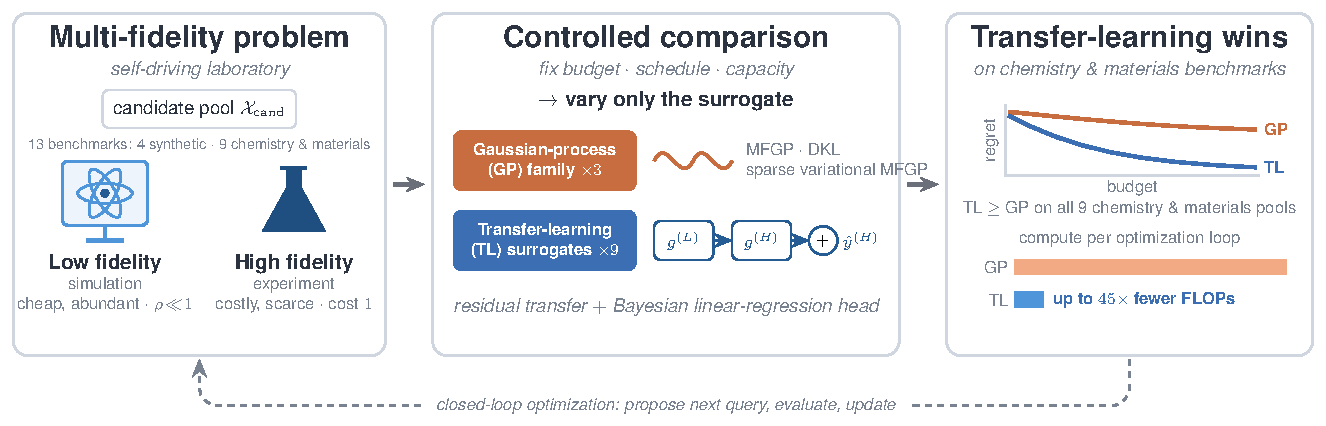
\includegraphics[width=0.9\textwidth]{paper_figures/fig1_overview.pdf}\\[1pt]
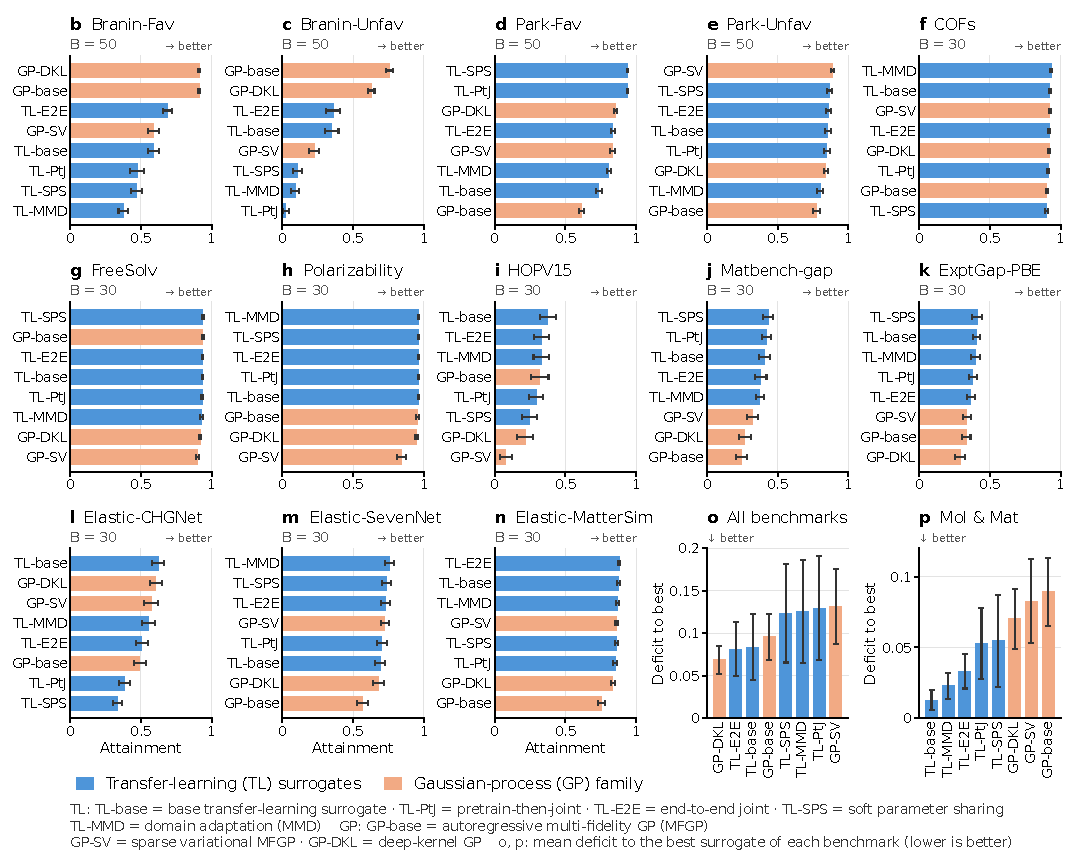
\includegraphics[width=\textwidth]{paper_figures/fig1_attainment.pdf}
\caption{Overview of the surrogate comparison and headline results.
\textbf{a,} in a self-driving laboratory, a shared candidate pool
$\mathcal{X}_{\mathrm{cand}}$ is queried through a cheap low-fidelity (LF)
source (cost $\rho \ll 1$) and a scarce, expensive high-fidelity (HF) experiment
(cost $1$). With the budget, fidelity schedule, initial design and candidate representation held fixed (the acquisition policy is matched separately, Supplementary Fig.~\ref{suppfig:acquisition}), only the surrogate is varied: a three-member Gaussian-process family (baseline MFGP, deep-kernel
GP, sparse variational MFGP) against five transfer-learning (TL) surrogates, in
which a network trained on
LF data, $g^{(L)}$, provides the representation on which a Bayesian linear-regression head, fitted to the HF observations, predicts the HF objective; a second network trained on the HF data, $g^{(H)}$, enters the training loss only (Methods).
\textbf{b--n,} attainment per benchmark: for each seed and each of four targets (regret at or below the pool's top 5, 2, 1 and 0.5\% thresholds), the fraction of the budget window, from the end of the initial design to the budget $B$ shown, spent at or below the target; attainment is the mean over the four targets (0, never reached; 1, reached at once). Bars, mean $\pm$ s.e.\ over 40 seeds (36 and 39 for the sparse variational MFGP on Branin-Fav and Branin-Unfav, where the remaining fits failed); TL surrogates in blue, the Gaussian-process family in salmon; surrogates sorted within each panel (higher is better). Budgets: 50 on the synthetic functions and 30 on the nine chemistry and materials pools. \textbf{o,} summary over the thirteen benchmarks and \textbf{p,} over the nine chemistry and materials benchmarks: within each benchmark the attainment of the eight surrogates is rescaled to a normalised score (0, worst surrogate; 1, best surrogate in that benchmark) and the scores are averaged across benchmarks (mean $\pm$ s.e.); surrogates sorted from best to worst. Abbreviations are given beneath the panels.
}
\label{fig:overview}\label{fig:final_regret}
\end{figure*}

Most MFBO methods remain rooted in Gaussian process (GP) surrogates whose strength lies in calibrated uncertainty estimation. Standard multi-fidelity Gaussian processes (MFGP) perform strongly in low-data regimes and provide uncertainty estimates, but their limitations become increasingly apparent
 in the high-dimensional and heterogeneous search spaces characteristic of molecular and materials discovery.  GP surrogates scale poorly as LF data accumulate~\citep{williams2006gaussian}, while kernel-based similarity assumptions can struggle to capture nonlinear, biased or location-dependent relationships between LF and HF signals~\citep{snoek2015scalable, seeger2004gaussian, perdikaris2017nonlinear}. This limitation is particularly important in SDLs, where LF sources are often imperfect experimental proxies: they may be strongly informative only in restricted regions of the design space, misleading near the optimum or weakly correlated with the final HF objective.

Here we test an alternative hypothesis: in high-dimensional multi-fidelity discovery, optimization performance is governed less by uncertainty calibration or global LF--HF correlation than by the surrogate's capability to learn useful representations of the design landscape. When LF and HF signals share structure, such representations support cross-fidelity transfer; when LF information is weak or biased, they can still improve optimization by providing a more expressive model of high-dimensional molecular and materials descriptors than fixed-kernel GPs. This reframes multi-fidelity optimization as a representation-learning problem, in which the central challenge is to identify which structures in inexpensive data remain informative for expensive HF decisions.

Transfer-learning surrogates provide a natural mechanism for this reframing. By learning representations
from abundant LF data and adapting them to sparse HF observations through targeted correction~\citep{yosinski2014transferable}, these models can capture cross-fidelity structure while retaining the expressive capacity needed for \emph{prediction} in complex molecular and materials descriptor spaces~\citep{buterez2024transfer}. Although transfer-learning models have advanced multi-fidelity molecular property prediction, deep surrogates have served as the decision-making engine of closed-loop MFBO only in bespoke engineering-design settings~\citep{li2020dnnmfbo}: MFBO in molecular and materials discovery has been developed around GP surrogates~\citep{sabanza2025best}, and transfer-learning architectures representing distinct mechanisms of knowledge transfer have not been systematically evaluated under controlled closed-loop conditions. It therefore remains unclear when transfer-learning surrogates outperform GP baselines, which transfer mechanisms are most effective and whether any advantage arises from better uncertainty estimates, better predictive means or improved representation of the design space.

We address these questions through a controlled benchmark study of eight multi-fidelity surrogates across thirteen synthetic, chemistry and materials optimization tasks. The comparison includes five transfer-learning
surrogates and three GP baselines: autoregressive
MFGP~\citep{kennedy2000predicting}, 
deep-kernel GP~\citep{wilson2016deep}, and sparse variational MFGP\citep{titsias2009variational, hensman2013gaussian}. All transfer-learning surrogates shared one structure: an LF network learns a representation from the abundant proxy data, a Bayesian linear head fitted in closed form to the sparse HF observations predicts the HF objective from that representation, and an auxiliary HF network, trained on the HF residuals in a composite arrangement related to multi-fidelity neural networks~\citep{meng2020composite}, enters the training loss but not the prediction.
The five surrogates share one backbone and differ only in how information is transferred between these stages, so that within the transfer-learning family the transfer mechanism, not the network size, is what varies. We evaluated all methods under a shared closed-loop optimization protocol and used matched-acquisition control to separate surrogate effects from acquisition-policy effects (Fig.~\ref{fig:overview}).

Our results show that GPs remain highly effective when their inductive bias matches the objective, but that on every molecular and materials benchmark considered here the best transfer-learning surrogate is at least as effective as the best GP, and more effective where the cheap proxy misorders the best candidates. The advantage is explained primarily by the quality of the transfer-learned predictive mean and by preservation of the near-optimal region, rather than by calibrated uncertainty or global LF--HF correlation alone. Transfer-learning surrogates also scale more favourably under the repeated model updates typical of SDL workflows with abundant LF data, suggesting that surrogate design for MFBO should emphasize scalable learned representations that transfer information across fidelities while adapting to biased, local or weak LF signals.



\section{Results}\label{sec:results}

We evaluated eight surrogates on thirteen benchmarks
(Table~\ref{tab:benchmarks}) under a shared fixed protocol (Methods). Performance was measured as simple regret on HF
evaluations as a function of cumulative cost, averaged over forty random seeds, with the failed-fit exceptions specified in Fig.~\ref{fig:final_regret}. Fig.~\ref{fig:final_regret} summarizes each run by its attainment, the fraction of the budget window spent at or below the pool's top 5, 2, 1 and 0.5\% regret thresholds, averaged over the four targets (Methods), so that a surrogate scores highly only if it reaches good candidates early and keeps them; the underlying regret trajectories are shown in Fig.~\ref{fig:regret_trajectory}.

\subsection{Gaussian processes perform best on smooth, low-dimensional
objectives}\label{sec:res-branin}

The Gaussian-process family achieved the highest attainment on both Branin scenarios, indicating that GP models remain highly effective when
their inductive bias matches the objective structure. On Branin-Fav (the favourable fidelity scenario; Methods) the deep-kernel GP and the baseline MFGP reached attainments of $0.91$ against $0.69$ for the best transfer-learning surrogate (End-to-End Joint Training), and on Branin-Unfav the baseline MFGP reached $0.76$ against $0.36$ (End-to-End Joint Training; Fig.~\ref{fig:final_regret}b,c); the baseline MFGP and deep-kernel GP curves lie below every transfer-learning curve over almost the whole run (Fig.~\ref{fig:regret_trajectory}a,b). This observation is consistent with the Mat\'{e}rn-5/2 kernel providing a strong smoothness prior for an analytically smooth, two-dimensional objective,
allowing the GP posterior to model the surface accurately from relatively few observations.
On the four-dimensional Park functions, simple regret rapidly approached zero for most methods after only a small number of HF evaluations (Fig.~\ref{fig:regret_trajectory}c,d), so attainment separates the surrogates only by how early they converge. On Park-Fav the two best transfer-learning surrogates (Soft Parameter Sharing $0.94$ and Pretrain-then-Joint $0.94$) achieved higher attainment than the best GP (the deep-kernel GP, $0.85$) and the baseline MFGP was last ($0.62$), whereas on Park-Unfav the best of each family were close (Soft Parameter Sharing $0.87$ against the sparse variational MFGP $0.89$; Fig.~\ref{fig:final_regret}d,e). The largest GP advantages on synthetic objectives were therefore on the smooth, two-dimensional Branin functions: GPs are highly competitive when the kernel prior matches the structure of the objective, but the advantage is problem-dependent rather than universal.

\subsection{Transfer-learning surrogates \texorpdfstring{match or outperform Gaussian processes}{match or outperform Gaussian processes} on molecular and materials
benchmarks}\label{sec:res-chem}

On the chemistry and materials benchmarks the picture changed. On covalent organic frameworks (COFs), solvation free energy (FreeSolv) and polarizability every surrogate attained between $0.84$ and $0.96$ and the best transfer-learning surrogate and the best GP differed by at most about $0.01$ (Fig.~\ref{fig:final_regret}f--h): these pools reach near-zero final regret across families and show only small attainment margins. On organic photovoltaics (HOPV15) the best transfer-learning surrogate (Frozen-representation transfer, $0.38$) achieved higher attainment than the best GP (the baseline MFGP, $0.32$) and the sparse variational MFGP was last ($0.08$), and on Matbench-gap every transfer-learning surrogate ($0.37$--$0.43$) achieved higher attainment than every GP ($0.25$--$0.32$), the best pair being Soft Parameter Sharing ($0.43$) against the sparse variational MFGP ($0.32$; Fig.~\ref{fig:final_regret}i,j).

On the four larger materials pools the margin was small but again favoured the best transfer-learning surrogate: $0.41$ (Soft Parameter Sharing) against $0.34$ (sparse variational MFGP) on ExptGap-PBE, and $0.62$ against $0.60$ (Frozen-representation transfer against the deep-kernel GP), $0.75$ against $0.72$ and $0.88$ against $0.86$ (Domain Adaptation and End-to-End Joint Training against the sparse variational MFGP) on the three elastic-modulus pools, which draw on one HF source but differ in both the candidate set and the LF source (CHGNet, SevenNet and MatterSim; $R^2 = 0.29$, $0.41$ and $0.80$); attainment was higher for both families on the pools whose LF source agreed better with the HF values, although, because the candidate sets and their HF ranges differ as well, this ordering cannot be attributed to LF quality alone (Fig.~\ref{fig:final_regret}k--n). Across the nine chemistry and materials benchmarks the best transfer-learning surrogate therefore matched or exceeded the best GP on every pool in mean attainment, and the normalised score summary places all five transfer-learning surrogates above the three GPs (Fig.~\ref{fig:final_regret}p).

Two observations help interpret this advantage. First, the baseline MFGP's Mat\'{e}rn-5/2 kernel imposes a
single global notion of smoothness, whereas the molecular descriptor space, compressed by principal
component analysis (PCA), can be non-stationary and the LF--HF discrepancy may vary strongly across input space, particularly near the optimum. In this setting, a stationary-kernel GP can misrank promising candidates, while a transfer-learning surrogate can learn task-adapted representations from the larger
LF dataset and correct them towards the HF objective with a linear head that has few parameters to fit from the sparse HF data. Second, the trajectories locate the gap late in the run rather than at the first HF evaluation (Fig.~\ref{fig:regret_trajectory}). On HOPV15 all surrogates start alike, but the Gaussian-process family stops improving after roughly 20 HF-equivalent units and ends at mean regrets of $2.3$ (baseline MFGP), $2.6$ (deep-kernel GP) and $3.3$ (sparse variational MFGP) at $B = 30$, whereas the best transfer-learning surrogates keep improving and end at $1.2$ (End-to-End Joint Training) and $1.3$ (Frozen-representation transfer; Fig.~\ref{fig:regret_trajectory}h). On Matbench-gap every surrogate retains nonzero mean regret at $B = 30$, but the transfer-learning surrogates pull ahead after roughly 15 units: the best two (Soft Parameter Sharing and Pretrain-then-Joint) end at mean regrets of $0.05$ and $0.06$ against $0.12$ for the baseline and sparse variational MFGPs (Fig.~\ref{fig:regret_trajectory}i). These trajectories are consistent with a more useful ranking of the remaining HF candidates by the best transfer-learning surrogates, but do not identify why the GP curves plateau. The HOPV15 result further bounds this interpretation. The LF signal has little global linear association with HF for this task
($R^2 = 0.02$), but this does not exclude useful local LF information. The improvement is consistent with a more useful predictive mean for these molecular descriptors; it does not by itself distinguish representation expressivity from LF-to-HF transfer. Where the LF signal is informative and already places the optimum near the top of its ranking (COFs, FreeSolv, polarizability), every family reaches near-zero final regret and the best-family attainment margins are small; the larger advantages of the transfer-learning surrogates are therefore observed on pools whose LF proxy misorders the best candidates.

Performance also depended on transfer mechanism. Averaged over the thirteen benchmarks, the normalised attainment score places all five transfer-learning surrogates above every GP (Frozen-representation transfer $0.76$ and End-to-End Joint Training $0.74$; deep-kernel GP $0.61$; baseline MFGP $0.44$; Fig.~\ref{fig:final_regret}o), but no single transfer mechanism dominates: Domain Adaptation is the weakest transfer-learning surrogate on Branin-Fav and Pretrain-then-Joint on Branin-Unfav, Soft Parameter Sharing is the weakest on Elastic-CHGNet, and Soft Parameter Sharing ($0.25$) and Pretrain-then-Joint ($0.29$) fall below the baseline MFGP ($0.32$) on HOPV15, whereas Frozen-representation transfer ($0.89$) and Domain Adaptation ($0.87$) lead the chemistry and materials summary (Fig.~\ref{fig:final_regret}p). The spread of scores among the transfer-learning surrogates ($0.63$--$0.76$) indicates that outcomes
depended not merely on using transfer learning but on how transfer was implemented.

Matbench-gap, the inorganic band-gap benchmark optimized towards a photovoltaic target of $1.4$~eV, is one of two benchmarks, alongside ExptGap-PBE, on which the families' mean attainments separate completely: at $B = 30$ the lowest transfer-learning attainment ($0.37$) exceeds the highest GP attainment ($0.32$; Fig.~\ref{fig:final_regret}j), and the best transfer-learning surrogates lead the regret trajectories over the second half of the budget window (Fig.~\ref{fig:regret_trajectory}i). Surrogate choice was therefore most consequential on the pools whose LF proxy misorders the best candidates (HOPV15, Matbench-gap and, to a lesser degree, the four large materials pools) and less consequential on the pools where every family reaches near-zero final regret, consistent with the difficulty analysis below.

\begin{figure*}[t]
\centering
%% Display item 2 of 6: regret trajectories on the 13 benchmarks (fig2_trajectories.pdf, letters a--m baked in).
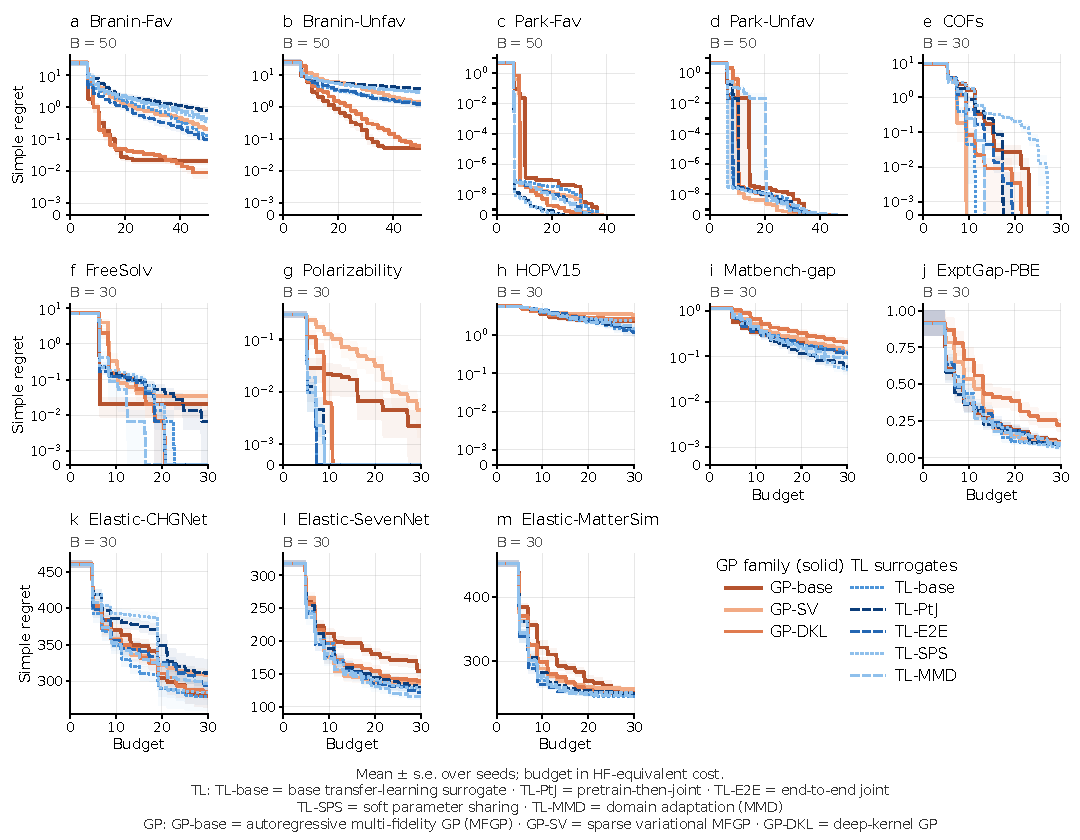
\includegraphics[width=\textwidth]{paper_figures/fig2_trajectories.pdf}
\caption{Regret trajectories as a function of cumulative budget (mean $\pm$ s.e.\ over 40
seeds; 36 and 39 for the sparse variational MFGP on Branin-Fav and Branin-Unfav); Gaussian-process family in solid orange lines, transfer-learning surrogates in dashed
and dotted blue lines, one panel per benchmark. Budget windows: 0--50 on the synthetic functions (\textbf{a}--\textbf{d}), on which every surrogate converges on the Park functions, and 0--30 on the nine chemistry and materials pools (\textbf{e}--\textbf{m}), the budgets of Fig.~\ref{fig:final_regret}. On the Branin functions the baseline MFGP and deep-kernel GP lead; on COFs every run reaches zero regret, whereas on FreeSolv and polarizability a few runs retain nonzero regret; on HOPV15 the transfer-learning surrogates keep improving after the Gaussian-process family has flattened, and on Matbench-gap they pull ahead over the second half of the window. Regret axes are logarithmic with zero shown at the floor; the four large-pool panels use linear axes because their regrets span about one decade or less. Abbreviations as in Fig.~\ref{fig:final_regret}.}
\label{fig:regret_trajectory}
\end{figure*}

\subsection{Optimum agreement, not global correlation, governs the transfer-learning
advantage}\label{sec:res-grid}

On the empirical benchmarks the global informativeness of the LF source and
its reliability near the optimum vary together, so either property could explain when
transfer learning wins. To examine their separate associations, we constructed a controlled grid on the
polarizability substrate in which curated LF sources vary the global LF--HF
$R^2$ and the top-10 optimum agreement independently, giving $126$ conditions of ten seeds each under
the standard optimization protocol; the GP family was split into the baseline MFGP and its variants (the deep-kernel and sparse variational MFGPs), and the three families --- all five transfer-learning surrogates, the baseline MFGP and its two variants, each family scored by its best member in each condition --- were compared pairwise on final
regret and on anytime performance, the area under the regret--budget curve (Methods).
The final-regret advantage maps are shown in Fig.~\ref{fig:family_heatmap}a--c.

\begin{figure*}[t]
\centering
%% Display item 3 of 6: controlled-grid final-regret advantage maps (fig3_grid_final_regret.pdf, letters a--c baked in).
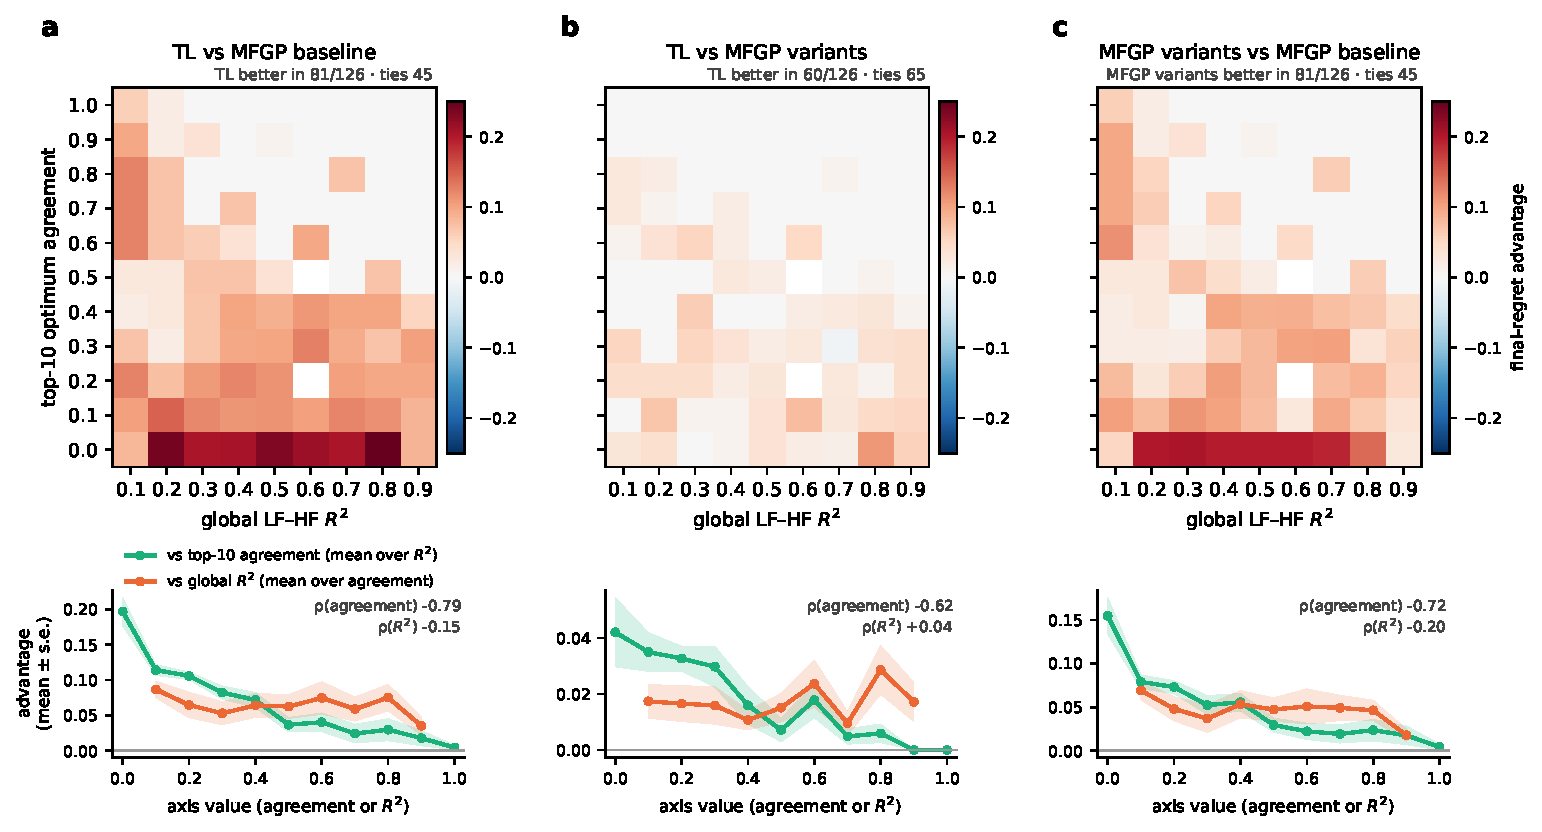
\includegraphics[width=0.95\textwidth]{paper_figures/fig3_grid_final_regret.pdf}
\caption{Family-split advantage maps from the controlled fidelity-quality grid (Methods). \textbf{a--c,} mean final-regret advantage of the best member of one family over the best member of another (second-named minus first-named family, in units of the HF range; blue favours the first-named family and orange the second-named) in bins of the global LF--HF $R^2$ (horizontal) and the top-10 optimum agreement (vertical): transfer learning (TL) against the baseline MFGP (\textbf{a}), TL against the MFGP variants (deep-kernel and sparse variational; \textbf{b}) and the MFGP variants against the baseline (\textbf{c}); $126$ conditions run for all five transfer-learning surrogates and all three Gaussian-process methods with ten seeds each, one colour scale shared by the three maps, and above each map the number of conditions favouring the first-named family and the number of exact ties. Lower row, the per-condition advantage against the top-10 agreement (mean over $R^2$) and against $R^2$ (mean over agreement), mean $\pm$ s.e., with the Spearman rank correlation $\rho$ of the $126$ per-condition advantages with each axis.}
\label{fig:family_heatmap}
\end{figure*}

Three observations emerge. First, the transfer-learning family --- the best of its five surrogates in each condition --- is never worse than the baseline MFGP anywhere on the plane: its final-regret advantage is positive in $81$ of $126$ cells and the remaining $45$ cells tie, every seed of the selected best members reaching the optimum (mean advantage $0.072$ in units of the HF range; Fig.~\ref{fig:family_heatmap}a). Second, the GP representative matters: against the MFGP variants the advantage narrows to $66$ cells, with $60$ ties and no reversal (mean $0.025$; Fig.~\ref{fig:family_heatmap}b), because the variants themselves improve on the baseline in $81$ cells (Fig.~\ref{fig:family_heatmap}c). Third, the advantage is organized primarily along the agreement axis rather than the $R^2$ axis: the per-cell advantage over the baseline correlates with the top-10 agreement (Spearman rank correlation $\rho = -0.81$) far more strongly than with $R^2$ ($\rho = -0.09$), falling from about $0.22$ at zero agreement to zero at full agreement while its profile against $R^2$ stays between $0.04$ and $0.09$ (lower row of Fig.~\ref{fig:family_heatmap}); against the MFGP variants the two dependences are $\rho = -0.78$ and $+0.11$. Within this grid, the transfer-learning advantage therefore tracks preservation of the best candidates more strongly than the global correlation commonly used to characterize an LF source.

\subsection{The advantage stems from the surrogate, not the acquisition
policy}\label{sec:res-acquisition}

Because the GP and transfer-learning surrogates used structurally different acquisition
policies under the default protocol, we matched the acquisition policy across both model families to test whether
the observed advantage of transfer-learning surrogates could be explained by this asymmetry. In the default setting, the baseline MFGP used an uncertainty-driven expected-improvement (EI) acquisition for the LF query whereas the transfer-learning surrogates used a greedy policy (Methods). We therefore compared matched acquisition settings by running the baseline MFGP under a greedy policy and the transfer-learning surrogates under an uncertainty-driven EI policy using their own Bayesian linear-regression (BLR) predictive standard deviation (Supplementary Fig.~\ref{suppfig:acquisition} shows End-to-End Joint Training). Using the greedy policy for the baseline MFGP had little effect on performance. Its attainment under the greedy policy was within $0.03$ of that under EI on eight of the nine benchmarks, and on HOPV15 the greedy policy lowered it ($0.23$ against $0.32$) rather than raising it, so the limitation of the baseline MFGP, where one appears, arises primarily from the surrogate rather than the acquisition policy. The transfer-learning surrogate was likewise insensitive to the acquisition policy: with its BLR uncertainty driving EI, End-to-End Joint Training attained within $0.01$ of its greedy value on seven benchmarks, $0.04$ less on Branin-Fav and $0.07$ more on HOPV15 (Supplementary Fig.~\ref{suppfig:acquisition}a--i); across the five transfer-learning surrogates the sign of the EI effect on HOPV15 depends on the surrogate (Supplementary Fig.~\ref{suppfig:acquisition}j).
These results suggest that the baseline MFGP
posterior \emph{mean} misranks the promising regions in these descriptor spaces, so changing the acquisition policy has limited effect. By contrast, the transfer-learning surrogate appeared to provide a more useful ranking of HF candidates, consistent with the surrogate contributing more to these differences than the LF acquisition policy under a fixed greedy HF rule. We therefore examined the role of exploration further using a broader acquisition-function portfolio.

%% The surrogate x acquisition comparison is Supplementary Fig. 1 (paper_figures/supp_acq_matrix.pdf).


\subsection{\texorpdfstring{Uncertainty-driven exploration adds little}{Uncertainty-driven exploration adds little}}\label{sec:res-uq}

Whether calibrated surrogate uncertainty improves BO depends on both the acquisition policy and the structure of the benchmark. To test this systematically, we replaced the greedy LF policy with a portfolio of five uncertainty-driven acquisitions spanning the standard taxonomy (the improvement-based EI and probability of improvement, the optimistic GP lower confidence bound, the information-theoretic max-value entropy search and sampling-based Thompson sampling; Methods), each using the BLR predictive standard deviation of the transfer-learning surrogate with its architecture, training configuration, fidelity schedule, HF protocol and random seeds held fixed, across all five transfer-learning surrogates and nine benchmarks (Supplementary Fig.~\ref{suppfig:portfolio}).

Uncertainty-driven exploration offered little improvement in mean attainment on these benchmarks. On COFs, FreeSolv and polarizability, no acquisition improved mean attainment over the greedy policy by more than a small margin: when the transfer-learned mean already provides a useful ranking, exploration has little to add. The acquisition family mattered more than the presence
of uncertainty alone. No uncertainty-driven acquisition raised the mean attainment of the transfer-learning surrogates by more than a small margin on any benchmark, whereas Thompson sampling lowered it markedly on HOPV15 and Matbench-gap and the lower confidence bound and max-value entropy search lowered it on the Branin functions (Supplementary Fig.~\ref{suppfig:portfolio}).
The greedy LF policy therefore remained a reliable default within this portfolio, and no uncertainty-driven acquisition offered a consistent benefit over it.

\begin{figure*}[tp]
\centering
%% Display item 4 of 6: calibration versus attainment on the 13 benchmarks (fig4_calibration_attain.pdf, letters a--m baked in).
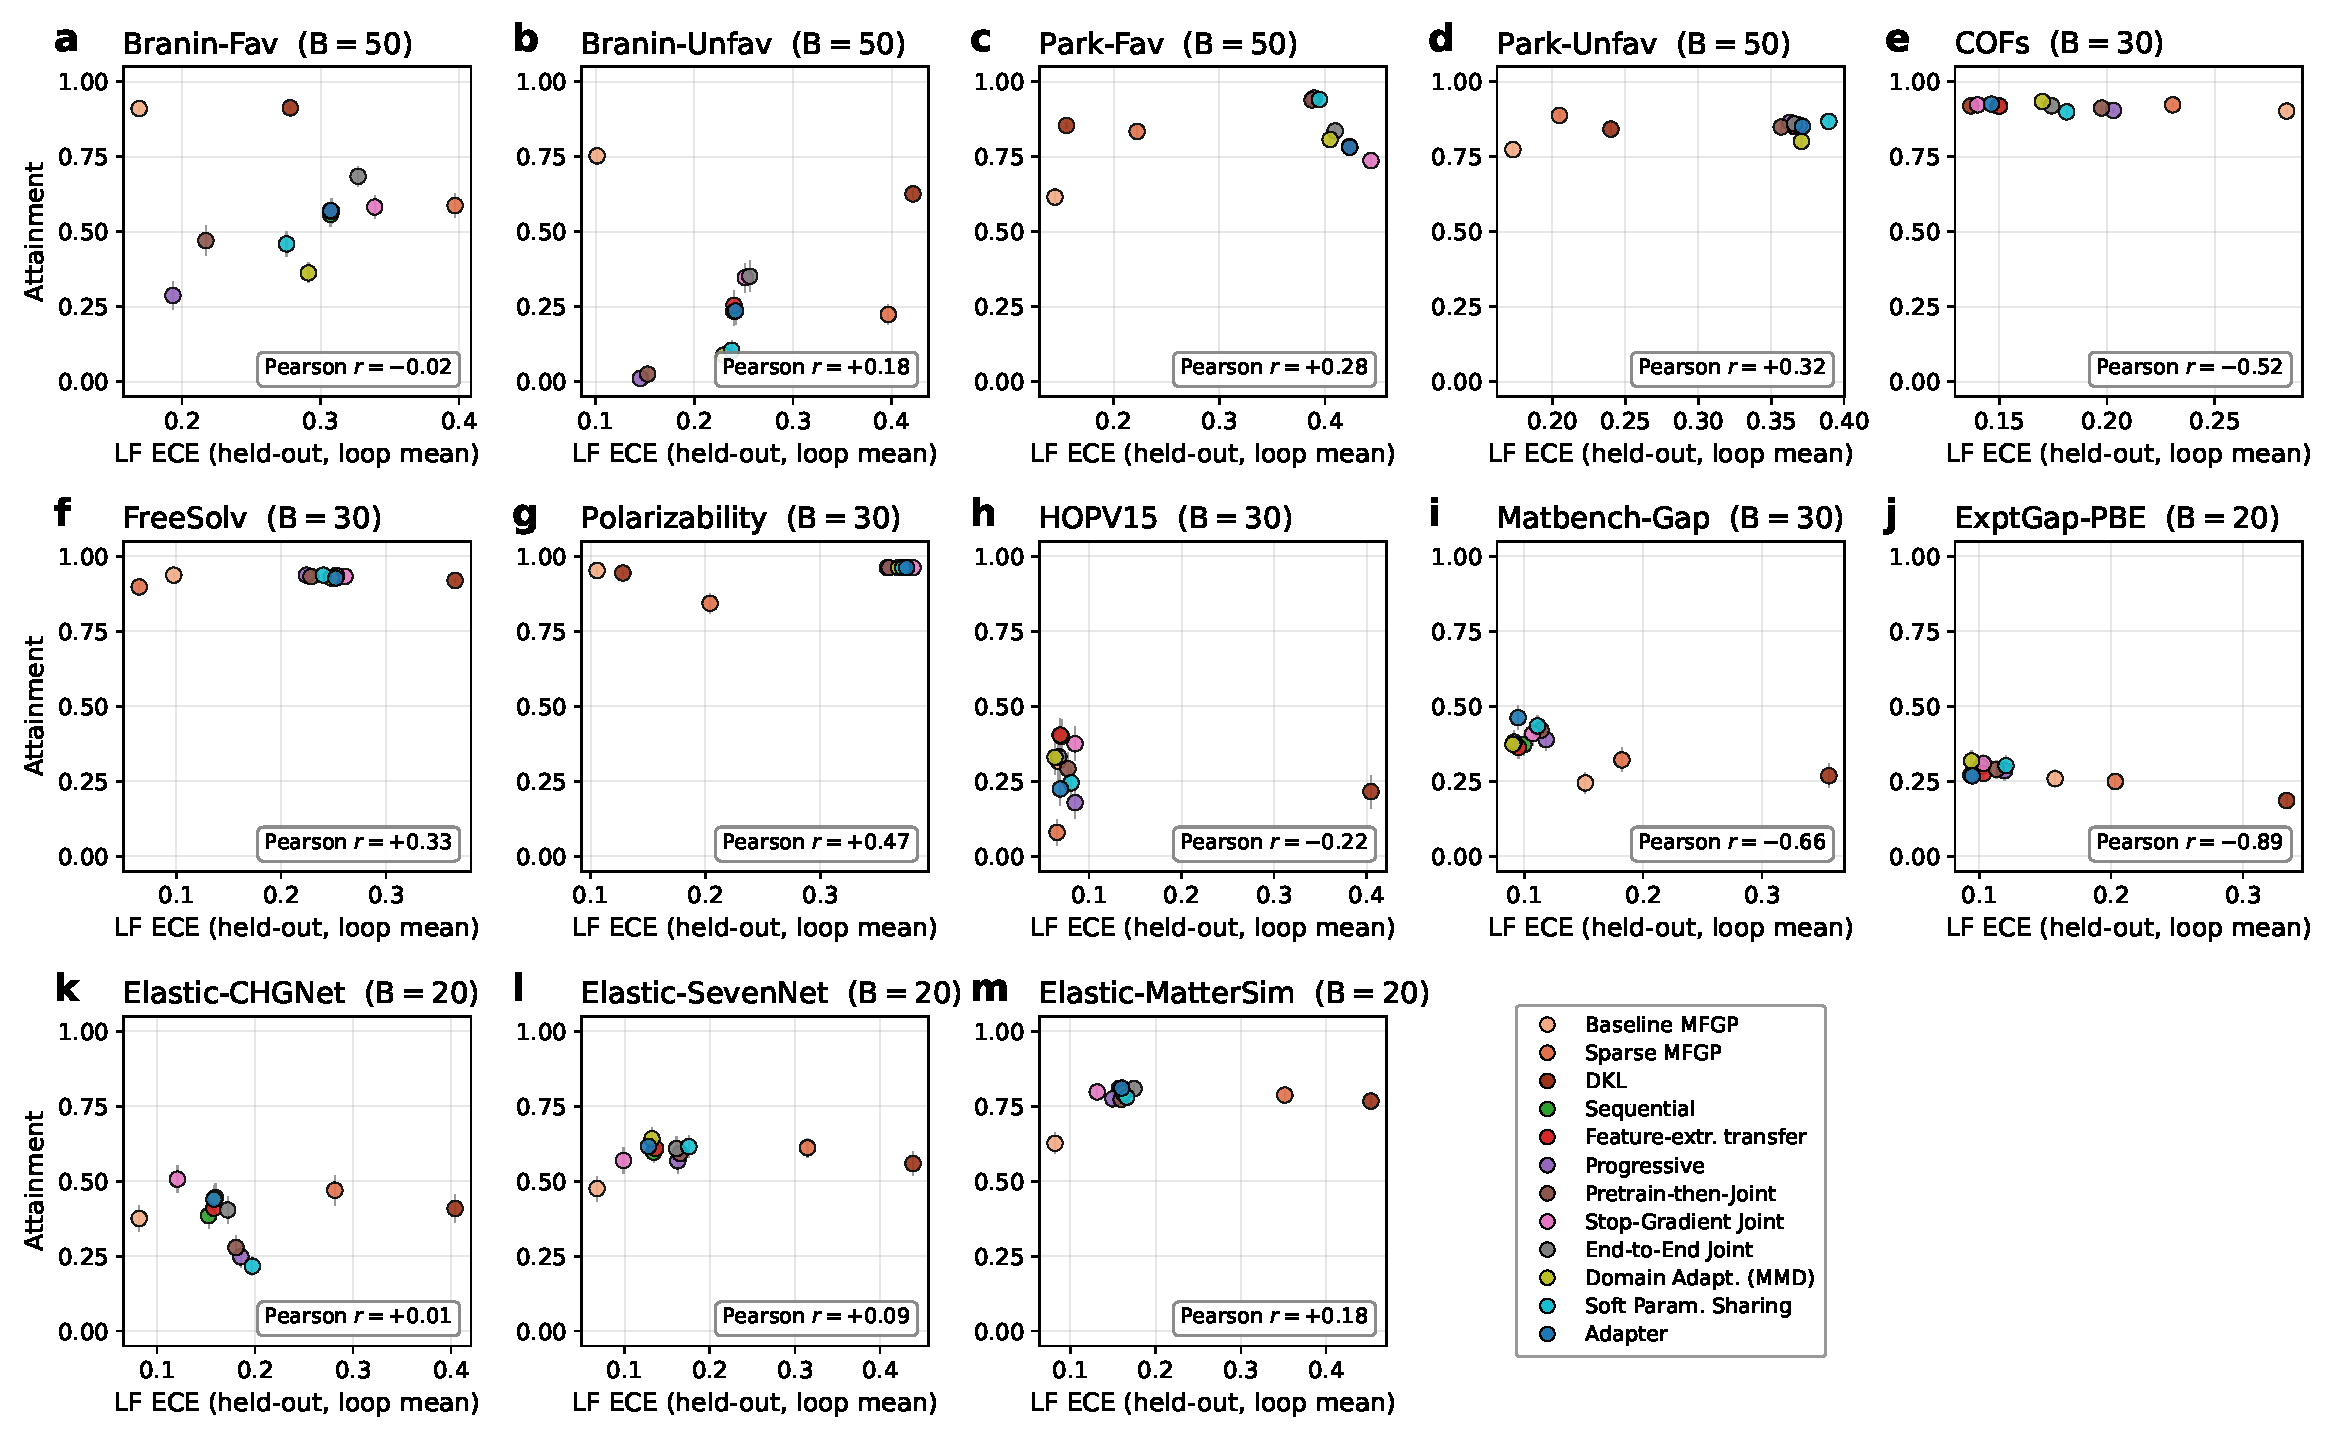
\includegraphics[width=0.9\textwidth]{paper_figures/fig4_calibration_attain.pdf}
\caption{Calibration does not predict optimization performance.
\textbf{a--m,} calibration versus attainment: each point is one of the eight surrogates (colour, family: Gaussian-process family in orange, transfer-learning surrogates in blue; marker, surrogate; legend), placed at its held-out low-fidelity expected calibration error averaged over the refits of the source runs (horizontal; Supplementary Note~\ref{suppnote:acquisition_variants}) and at its attainment from Fig.~\ref{fig:final_regret} at the budget shown (vertical; mean $\pm$ s.e.\ over 40 seeds, except 36 and 39 for sparse variational MFGP on Branin-Fav and Branin-Unfav), one panel per benchmark. The Pearson correlation across the eight surrogate means is given for description only (higher attainment is better, so a negative $r$ associates lower calibration error with better optimization). No consistent relation appears: $|r| \ge 0.5$ only on Matbench-gap and ExptGap-PBE (\textbf{i},\textbf{j}), where the three GP surrogates are both the worst-calibrated and the least effective; on COFs, FreeSolv and polarizability (\textbf{e}--\textbf{g}) every surrogate attains $0.84$--$0.96$ and the small attainment range limits interpretation of the correlation.}
\label{fig:calibration}
\end{figure*}

Calibration quality was a poor predictor of optimization performance: across the eight surrogates and thirteen benchmarks, the correlation between the loop-mean held-out LF calibration error and attainment had no consistent sign, and exceeded $|r| = 0.5$ only on Matbench-gap and ExptGap-PBE ($r = -0.67$ and $-0.90$), where the three GP surrogates were both the worst-calibrated LF models (calibration error $0.15$--$0.36$ against $0.08$--$0.12$ for the transfer-learning surrogates) and the weakest optimizers; on COFs, where every surrogate attains $0.90$--$0.93$, the small attainment range limits interpretation of the correlation ($r = -0.48$) (Fig.~\ref{fig:calibration}a--m). Nor did good calibration mark the best optimizers: the baseline MFGP had the lowest LF calibration error on seven of the thirteen benchmarks yet ranked in the lower half of the eight surrogates by attainment on seven of the nine chemistry and materials pools, whereas the deep-kernel GP, the worst-calibrated on eight benchmarks, was among the best optimizers on Branin.
 Together, these results are consistent with an advantage in the transfer-learned mean under the tested acquisition policies, with uncertainty-driven exploration adding little. The LF calibration analysis does not directly assess the HF uncertainty used by the acquisition portfolio.

\subsection{When is a surrogate necessary?}\label{sec:res-topk}

A learned surrogate is not equally valuable for every optimization problem. To identify when surrogate learning adds benefit, we compared the optimization outcomes with a surrogate-free screen that ranks candidates by their LF
value and evaluates the single top-ranked candidate at HF. The resulting deterministic screening
regret provides a reference for whether the LF proxy alone identifies a good candidate; it is not a budget-matched optimization baseline
(Fig.~\ref{fig:topk}). This analysis separated the benchmarks into two regimes by their screening regret (Regime~A, at most $0.3$; Regime~B, above $0.3$, in each pool's stored objective units). This is a descriptive split, not a common accuracy tolerance across tasks. In Regime~A, represented by Park-Fav and polarizability, the top LF
candidates coincide almost exactly with the top HF candidates. The top-1\% overlap was approximately $1$ and the screening regret was no greater than $ 0.09$. In these examples, the LF screen already identified a near-optimal candidate. In Regime~B, represented by COFs and
Branin, high global LF--HF correlation conceals poor agreement among the top-ranked  candidates. COFs had a
Spearman rank correlation $\rho$ of $0.998$ but a screening regret of $4.52$. In this setting, surrogate-based optimization improved on the single-candidate screen; every surrogate reached zero regret within the budget (Fig.~\ref{fig:regret_trajectory}e), substantially outperforming the surrogate-free screen. COFs and polarizability both had $R^2 \approx 0.96$ or higher but had different screening outcomes, so the need for a surrogate depends less on global LF--HF correlation than on whether the LF proxy preserves the near-optimal region. The
best transfer-learning surrogates reached similarly low regret where the screen was near-optimal and improved on this screen where the LF ranking was less useful. Both HOPV15 and Matbench-gap fall in
Regime~B. An LF screen produced a regret of $3.90$ on HOPV15 where the Scharber proxy
was nearly uninformative and $0.91$ on Matbench-gap. The four larger materials pools fall in Regime~B as well. On ExptGap-PBE the screen misses the optimum by $1.15$~eV (the first indexed HF optimum sits at LF rank $1{,}033$ of $3{,}508$), and on the three elastic-modulus pools the screening regret is $384$~GPa with the CHGNet source and $369$~GPa with SevenNet ($74\%$ and $97\%$ of the respective HF ranges) but $3$~GPa with MatterSim ($0.6\%$ of the range, the HF optimum at LF rank 2), so these three related pools span the whole range from a useless to a nearly sufficient screen (Fig.~\ref{fig:topk}a,b). These results show scope to improve on the single-candidate screen, and on HOPV15 and Matbench-gap the choice of surrogate matters as well (Fig.~\ref{fig:final_regret}i,j).

\begin{figure*}[tp]
\centering
%% Display item 5 of 6 — composite: (a,b) top-k overlap and LF-only screening
%% regret; (c) compute scaling law. Together: when a learned surrogate is
%% needed, and what it costs. Panel letters baked into the PDFs.
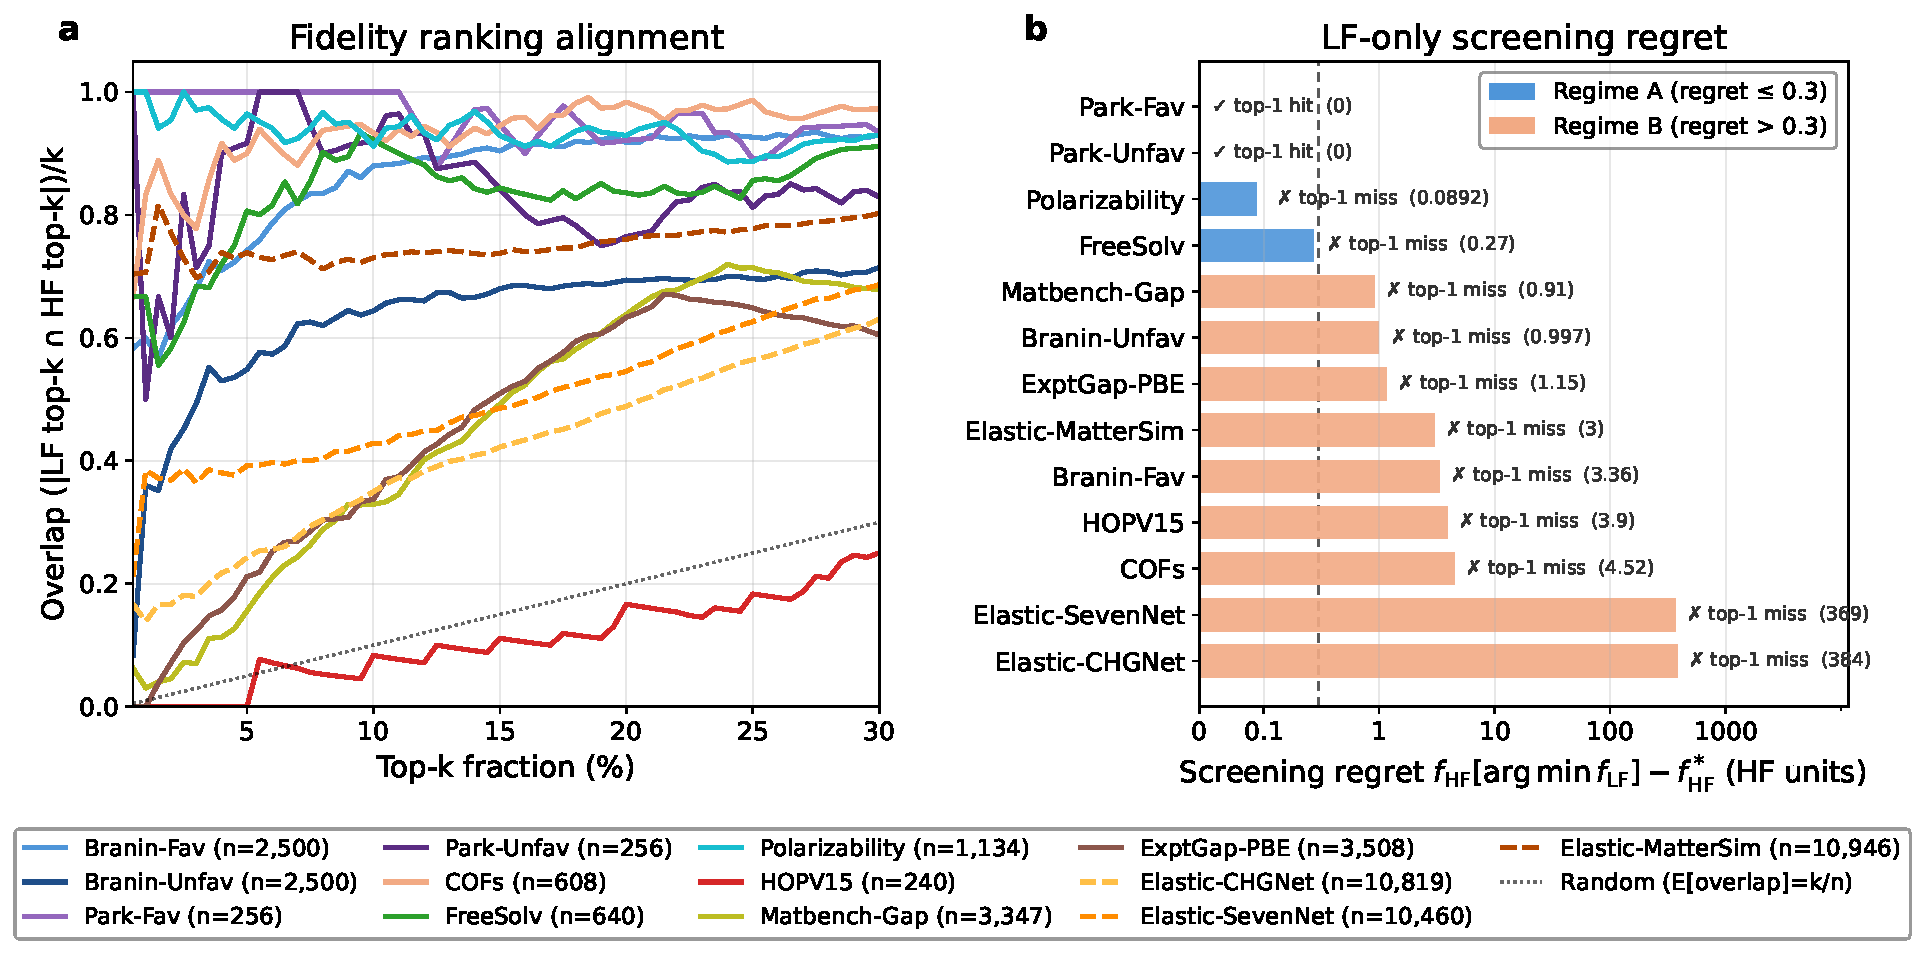
\includegraphics[width=0.92\textwidth]{paper_figures/B2_topk_13.pdf}\\[6pt]
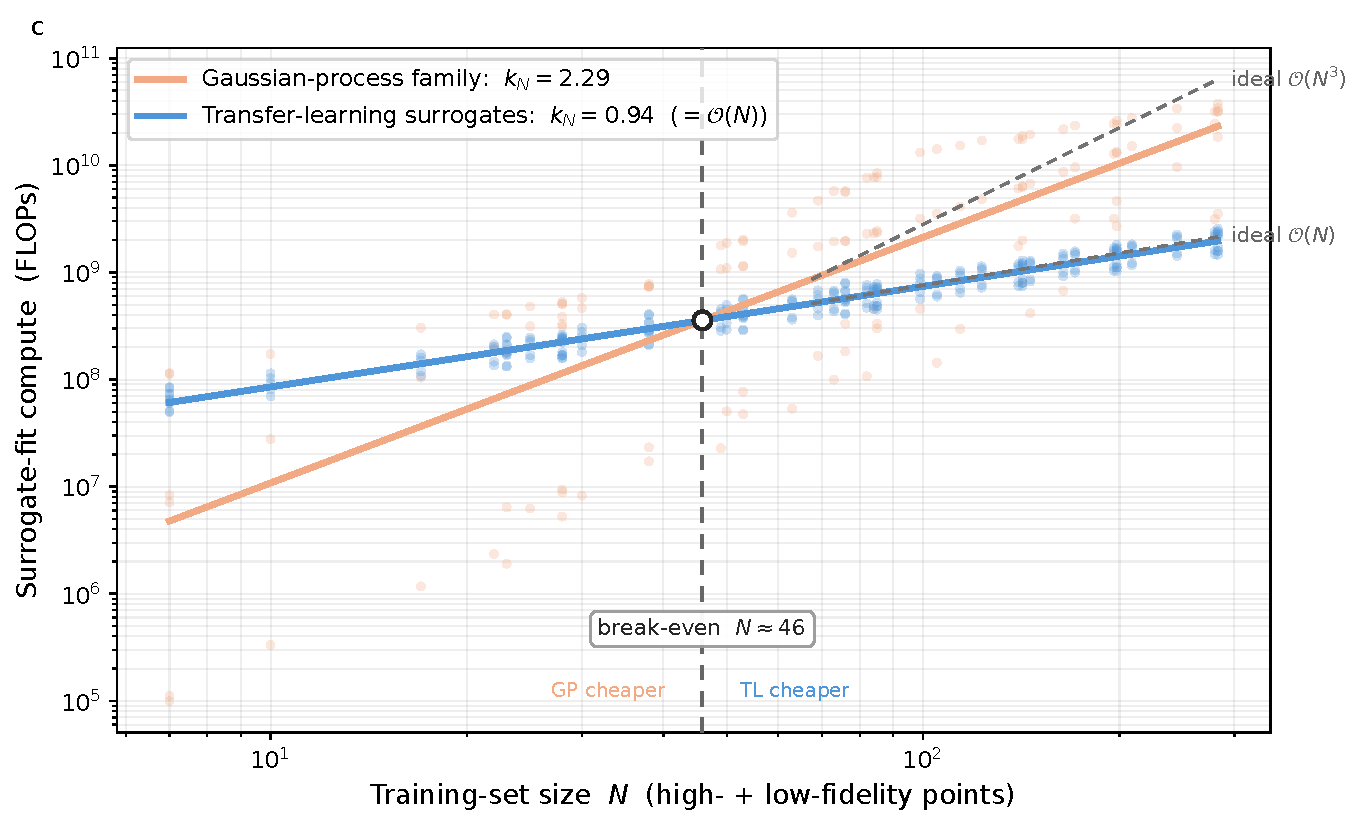
\includegraphics[width=0.85\textwidth]{paper_figures/compute_scaling_law_blr.pdf}
\caption{When a surrogate is needed, and what it costs.
\textbf{a},\textbf{b,} task difficulty and the need for a surrogate. Top-$k$ overlap
between the low- and high-fidelity rankings (\textbf{a}) and the resulting LF-only
screening regret (\textbf{b}) for each of the thirteen benchmarks, defined as $f_H(\arg\min f_L)-\min f_H$ for one LF-selected candidate, with ties resolved by first index. Regret is in each pool's stored objective units and is drawn on a symmetric-logarithmic axis; the dashed Regime boundary at $0.3$ is descriptive. High global correlation does not
guarantee top-$k$ overlap: Regime~B identifies failure of this single-candidate screen, while Regime~A identifies low screening regret under this convention. The four larger materials pools all fall in Regime~B: the screen misses the optimum by $1.15$~eV on ExptGap-PBE and by $384$, $369$ and $3$~GPa on the CHGNet, SevenNet and MatterSim elastic-modulus pools.
\textbf{c,} computational scaling law across nine of the thirteen benchmarks (the four large materials pools are not profiled), for the surrogates of Figs.~\ref{fig:final_regret} and~\ref{fig:regret_trajectory} (BLR head included). Each point is
the median surrogate-fit compute (hardware-independent floating-point operations, FLOPs) of one surrogate on one
benchmark at one budget fraction, placed at the training-set size $N$ (high- plus
low-fidelity points) it was fitted on; salmon, Gaussian-process family; blue,
transfer-learning surrogates (the five transfer-learning surrogates). A shared-slope power-law fit gives $k_N = $$0.94$
(fit $R^2 = $$1.00$, close to $\mathcal{O}(N)$) for the transfer-learning surrogates
and $k_N = $$2.29$ (fit $R^2 = $$0.93$) for the Gaussian-process family, which lies below pure
cubic because it includes the sparse variational MFGP and the deep-kernel GP, with the exact baseline MFGP approaching the ideal $\mathcal{O}(N^3)$ (faint dashed guides). The two family
laws cross at a break-even size $N \approx $$46$ (vertical line): below it the Gaussian
processes are cheaper to fit, above it the transfer-learning surrogates are cheaper by
a margin that grows with $N$, reaching roughly $2.9\times$ at $N = 100$ and $7.4\times$ at $N = 200$. Absolute per-benchmark FLOPs and the average compute ranking are in
Supplementary Fig.~\ref{suppfig:computing_time} (Supplementary
Note~\ref{suppnote:computational_cost}).}
\label{fig:topk}\label{fig:scaling_law}
\end{figure*}

\subsection{Computational cost}\label{sec:res-cost}

We quantified computational cost in floating-point operations (FLOPs) on nine benchmarks, profiling one surrogate fit and one pool-wide prediction at five training-set sizes for two seeds (42--43), then interpolating these costs over the optimization loop. FLOPs isolate algorithmic scaling from implementation and hardware effects, although they do not capture memory footprint, which is particularly relevant for the sparse variational MFGP's inducing-point overhead, or engineering factors such as parallelization and library-level optimization that affect wall-clock cost in deployment. Profiled for the surrogates of Figs.~\ref{fig:final_regret} and~\ref{fig:regret_trajectory}, that is, with the BLR head and the unused residual network included, the transfer-learning surrogates scaled almost linearly with the number of observations (fit-FLOP exponent $k = $$0.9$--$1.0$), reflecting fixed-architecture training, whereas the exact baseline MFGP scaled cubically ($k = 3.0$), consistent with exact inference and marginal-likelihood optimization; the sparse variational MFGP and the deep-kernel GP had intermediate exponents ($k = 2.3$ and $1.5$) but the largest constant factors (Fig.~\ref{fig:scaling_law}). The family-level cost curves crossed at $N \approx $$46$, below which the GPs were cheaper to fit and above which the transfer-learning surrogates were cheaper by a margin that grew to approximately $2.9$ times at $N = 100$ and $7.4$ times at $N = 200$.

Integrated over the optimization loop, the sparse variational MFGP and the deep-kernel GP were the most expensive surrogates on every profiled benchmark, requiring up to approximately $22$-fold and $15$-fold more FLOPs than the fastest transfer-learning surrogate (for the sparse variational MFGP, $5.0$ versus $0.23$ TFLOPs on FreeSolv at $B = 50$), and the baseline MFGP up to $5.6$-fold, with the gap widening as the evaluation budget grew (Supplementary Note~\ref{suppnote:computational_cost}, Supplementary Fig.~\ref{suppfig:computing_time}); on the smallest pools and budgets, such as HOPV15 and Park-Unfav, the cubic cost of the baseline MFGP remained negligible and it was the cheapest surrogate of all. Under the fixed optimization protocol, transfer-learning surrogates therefore combined attainment matching or exceeding the best GP on every chemistry and materials benchmark with more favourable computational scaling, which matters in SDL settings where abundant LF data and repeated surrogate updates make retraining cost a significant component of the closed loop.

\section{Discussion}\label{sec:discussion}

By bringing transfer learning into the multi-fidelity optimization loop, we find a
transfer-learning surrogate to be the better engine for molecular and materials
discovery: within our protocol the choice of surrogate, more than the acquisition policy, governs MFBO performance in
high-dimensional molecular and materials spaces.
Across thirteen benchmarks the GP family achieved the highest attainment only on the two smooth, low-dimensional Branin functions and, by $0.02$, on Park-Unfav; on every chemistry and materials pool the best transfer-learning surrogate matched or exceeded the best GP, with the clearest margins on the pools whose LF proxy misorders the optimum (HOPV15, Matbench-gap) and small attainment margins where every family reaches near-zero final regret (COFs, FreeSolv, polarizability). The practical implication for SDLs is
direct: on descriptor-based molecular and materials pools, a transfer-learning
surrogate is a more reliable default than the baseline MFGP, and on evaluation-rich tasks it delivers this accuracy at up to roughly $22\times$ fewer FLOPs than the most expensive GP in the separate nine-task compute profiles.

Uncertainty-driven exploration, by contrast, produced no winner: no acquisition in the portfolio improved consistently on the greedy policy, although some acquisitions substantially lowered attainment. Where the LF signal transfers strongly and cleanly (COFs, FreeSolv, polarizability), the transfer-learning surrogates reach near-zero regret by greedily exploiting their transfer-learned mean, and gains in mean attainment were small when a five-acquisition portfolio used BLR uncertainty for LF exploration instead. Where exploration increased mean attainment, the gains were small, whereas Thompson sampling lowered attainment on HOPV15 and Matbench-gap and was the least reliable acquisition.
Calibration quality did not consistently predict optimization performance; on Matbench-gap and ExptGap-PBE, the negative correlations coincided with poorly calibrated GP surrogates also being the weakest optimizers. We interpret this through the strong-transfer regime that often characterizes SDL pipelines: when an abundant LF signal already orders candidates well, a high-quality posterior mean is worth more than exploration, and exploration adds little. Effort is therefore better spent first on the quality of the transferred representation.

The benchmark also clarifies when a learned surrogate is needed at all. Our
screening-regret analysis separated tasks in which a surrogate-free LF screen is
near-optimal (Regime~A) from those in which it fails despite a high global correlation
(Regime~B), and showed that regime membership cannot be inferred from the correlation
alone.

The controlled fidelity-quality grid adds a methodological caution and sharpens this
claim. The apparent size of the transfer-learning advantage depends on which member
represents the GP family: against the baseline MFGP alone, transfer
learning, taken as the best of the five surrogates in each condition, is never worse in mean final regret and wins in $81$ of $126$ conditions, whereas against the stronger variants the final-regret gap
narrows by about two thirds and what survives is robustness
precisely where the LF source misorders the best candidates. Comparisons of
learned surrogates against ``Gaussian processes'', in our study and in the wider
literature, should therefore be read against the strength of the chosen
representative. The grid also locates our conclusions relative to guidance built on
global fidelity correlation~\citep{sabanza2025best}: because the advantage is organized primarily along the optimum-agreement axis and depends only weakly on $R^2$, a decision map indexed by global correlation alone cannot separate the conditions in which a
learned surrogate is essential from those in which it is dispensable. The scope of
this evidence is deliberately narrow, a mechanism experiment with curated
LF sources on a single substrate, whose synthetic degradations need not mirror
real experimental or simulation biases; the benchmark suite, not the grid,
carries the generalization claim.

Several limitations bound these conclusions and motivate future work. Our protocol is
restricted to two fidelity levels with a deterministic round-robin schedule that reflects
the parallel-resource structure of many SDLs but does not exercise adaptive, cost-aware
fidelity selection; the composite training structure and the linear head extend naturally to hierarchical
fidelities, which we leave to future work. The transfer-learning surrogates use fixed, modest-capacity
multilayer perceptrons on precomputed descriptors reduced by PCA;
larger architectures or learned molecular representations could further widen the gap but
were deliberately excluded to keep the comparison fair. The comparison also leaves the
transfer-learning hyperparameters fixed while the GP baselines re-fit their kernel
hyperparameters by marginal-likelihood maximization at every iteration; this asymmetry
is conservative where transfer learning wins, but the GP advantage on the smooth synthetic objectives should be read with it in mind. The predictive uncertainty of the transfer-learning surrogates likewise comes from BLR heads whose precisions are either fixed ($\alpha = \beta = 1$ for the LF head used in the calibration analysis) or set by a leave-one-out rule (the HF head that drives the acquisition portfolio), not calibrated per benchmark, and the HF head treats the LF representation as a fixed basis although, in Pretrain-then-Joint, End-to-End Joint and Soft Parameter Sharing, that representation has itself been trained on the same HF values, which makes the HF predictive variance of these three surrogates optimistic, so the limited value of uncertainty-driven exploration reported here is specific to that construction; better-calibrated or ensemble-based uncertainty could shift the balance. Our evaluation is also retrospective,
optimizing over fixed candidate pools that emulate the closed loop rather than driving a live
autonomous platform, so the surrogate ranking we report remains to be confirmed in
deployment. Finally, the comparison is against
the baseline MFGP and the two MFGP variants rather than the entire space
of GP methods, so our claims are scoped to this widely used family under a
pool-based, two-fidelity protocol.

Taken together, these results establish transfer-learning surrogates as the surrogate
of choice for molecular and materials multi-fidelity optimization, and yield a concrete
recipe for the engine at the core of an SDL: default to a transfer-learning surrogate on descriptor-based
molecular and materials pools, reserve GPs for the smooth, low-dimensional
design spaces where their inductive bias is an asset, and invest first in the quality of the
transferred mean, treating uncertainty-driven exploration as a secondary concern. Because this guidance
concerns the surrogate rather than the acquisition policy or fidelity schedule, it can be
adopted within existing autonomous-experimentation platforms with no change to their optimization policy.


\section{Methods}\label{sec:methods}

\subsection{Problem setup}\label{sec:meth-setup}

We considered the problem of MFBO for minimizing an expensive
HF objective under a finite experimental budget.  The HF
function $f^{(H)} : \mathcal{X} \to \mathbb{R}$ represents the target objective over a compact design space $\mathcal{X} \subseteq \mathbb{R}^d$ with the aim of identifying the global minimizer $x^\star = \arg\min_{x \in \mathcal{X}} f^{(H)}(x)$. A
cheaper LF function $f^{(L)}$ provides biased but potentially informative observations of the same landscape at reduced cost. We characterized the informativeness of the LF source by its squared Pearson correlation with the HF objective over the candidate pool, $R^2 =
\mathrm{Corr}(f^{(L)}(x), f^{(H)}(x))^2$, referred to as the global LF--HF $R^2$ (for the synthetic functions, over $1{,}000$ uniform samples; Supplementary Note~\ref{suppnote:synthetic_functions}). Evaluation cost was modelled as $c_H = 1$ for
HF and $c_L = \rho$ for LF with $\rho \ll 1$. At each step, the optimizer selected a design point 
$(x_t, s_t)$ and a fidelity level $s_t \in \{L, H\}$ subject to the total budget constraint $\sum_t c_{s_t} \le B$. The 
performance was measured using the simple regret over HF evaluations, $r_T = \min_{t:
s_t = H} f^{(H)}(x_t) - f^{(H)}(x^\star)$.

\subsection{Pool-based optimization loop and acquisition}\label{sec:meth-loop}

Optimization was performed over a fixed candidate pool $\mathcal{X}_{\mathrm{cand}}$, with regret measured relative to its minimum HF objective value. A candidate already evaluated at a given fidelity was excluded from further queries at that fidelity only, so a candidate screened at LF remained available for HF evaluation. The initial design comprised two HF points and LF points of about the same total cost (5 to 25 points, depending on $\rho$), 3 to 4.5 HF-equivalent units in all, and was generated by furthest-point
sampling on every pool. At each iteration, the surrogate model was retrained
de novo on all accumulated observations. A deterministic round-robin
schedule issued $n_{\mathrm{LF}\rightarrow\mathrm{HF}} = \lfloor 1/\rho \rfloor$
LF queries between successive HF queries, isolating surrogate quality
from cost-aware fidelity heuristics and reflecting SDL pipelines in which LF and HF instruments operate in parallel. For the GP baselines, LF candidate selection used EI~\citep{jones1998efficient},
\begin{equation}\label{eq:ei}
\begin{aligned}
\alpha_{\mathrm{EI}}(x) &= (\hat{y} - \mu(x) - \xi)\,\Phi(Z) + \sigma(x)\,\phi(Z), \\
Z &= \frac{\hat{y} - \mu(x) - \xi}{\sigma(x)},
\end{aligned}
\end{equation}
where $\hat{y}$ is the best observed HF value, $\xi = 0.01$~\citep{snoek2012practical}, and $\Phi$, $\phi$ denote the
standard normal CDF and PDF respectively. The acquisition function was maximized by enumeration over the pool. For the
GP baselines, query locations at both fidelity levels were selected using the cross-fidelity posterior evaluated at the
HF level, which provides a predictive standard deviation in closed
form. The LF query maximized EI on this posterior with the HF incumbent, whereas the HF query, as for every surrogate in the study, took the candidate with the lowest predicted HF mean among those not yet evaluated at HF. For the transfer-learning surrogates, the main results used the greedy policy: both LF and HF candidates were selected by the minimum predicted HF mean $\mu^{(H)}$ among the candidates not yet evaluated at that fidelity. To assess sensitivity to uncertainty modelling, we evaluated several uncertainty-driven acquisition policies.  These included a portfolio of five acquisitions for the LF query, each evaluated on the predictive mean and BLR standard deviation of the HF prediction with the HF incumbent: EI, probability of
improvement~\citep{kushner1964new}, the GP lower confidence
bound~\citep{srinivas2012information}, max-value entropy search~\citep{wang2017max}, and
Thompson sampling~\citep{russo2018tutorial}, spanning the standard acquisition-function
taxonomy~\citep{shahriari2015taking}. The portfolio is analysed in
the Results (Supplementary Fig.~\ref{suppfig:portfolio}) and reported in full in the Supplementary
Information. All objectives were formulated as minimization problems, with maximization
targets negated.

\subsection{Surrogate models}\label{sec:meth-surrogates}

Our GP baselines covered standard, learned-feature, and
sparse-variational regimes of multi-fidelity GP modelling. The baseline MFGP was implemented using the
\texttt{SingleTaskMultiFidelityGP} in \texttt{BoTorch}~\citep{balandat2020botorch}, corresponding to an
autoregressive Kennedy--O'Hagan formulation~\citep{kennedy2000predicting} with a Mat\'{e}rn-5/2 kernel and fidelity
encoded as a binary indicator. Hyperparameters were fitted by exact
marginal-likelihood maximization with L-BFGS-B under the default priors of BoTorch 0.10.0, in double precision. The deep-kernel GP~\citep{wilson2016deep} replaces the conventional kernel with one
defined on neural network features trained jointly with the marginal-likelihood optimization (a network of widths 64, 64 and 16 with $\tanh$ activations feeding an RBF kernel with automatic relevance determination and a two-level index kernel, optimized for 500 Adam steps in single precision). The sparse
variational MFGP approximated the multi-fidelity posterior using variational
inference over up to 100 learned inducing points with a multi-task index kernel, optimized for 500 Adam steps on the full-batch evidence lower bound in single precision, providing a scalable alternative to
exact GP inference~\citep{titsias2009variational, hensman2013gaussian}. The transfer-learning surrogates were trained as two networks, a composite structure of the kind used in multi-fidelity neural networks~\citep{meng2020composite}, in which an LF network $g_{\theta}^{(L)}:\mathbb{R}^d\to\mathbb{R}$ and an
HF residual network $g_{\phi}^{(H)}:\mathbb{R}^{d+1}\to\mathbb{R}$ (conditioned
on the input and the LF prediction) combine in the training loss as
\begin{equation}\label{eq:residual}
\text{}\mu^{(H)}_{\mathrm{aux}}(x) = g_{\theta}^{(L)}(x) + g_{\phi}^{(H)}\!\left([x,\, g_{\theta}^{(L)}(x)]\right).
\end{equation}

The HF loss of every transfer mechanism is the squared error of $\mu^{(H)}_{\mathrm{aux}}$ on the HF observations, so the residual network is trained to fit the discrepancy $\delta(x) = f^{(H)}(x) - g_{\theta}^{(L)}(x)$ and, where the mechanism lets the HF loss reach $\theta$, the HF data shape the LF representation through it. Both networks were two-layer multilayer perceptrons of hidden width 64 with
$\tanh$ activations. The HF prediction, however, is not the output of the residual network. A run starts with two HF observations and ends with at most a few tens, for which a 64-unit two-layer network fitted to the HF residuals is heavily over-parameterized, and a point-estimate network provides no predictive variance for the acquisition functions. The prediction is therefore made by a Bayesian linear regression (BLR) head on the final-layer representation of the LF network, an adaptive-basis construction in the spirit of DNGO~\citep{snoek2015scalable,gawlikowski2023survey} in which the basis is the LF representation, learned from the abundant LF data, rather than the features of a network trained on the target data, and the HF adaptation is a closed-form linear read-out with 66 coefficients. The HF prediction is $\mu^{(H)}(x) = g^{(L)}_{\theta}(x) + w^{\top}[\,g^{(L)}_{\theta}(x),\, \varphi^{(L)}(x),\, 1\,]$, where $\varphi^{(L)}$ is the final-layer representation of the LF network and the weights $w$ are fitted in closed form to the HF residuals $y^{(H)} - g^{(L)}_{\theta}(x)$. For at least four HF observations, the ratio of prior to noise precision of the representation block is selected by leave-one-out error over $\{10, 30, 100, 300, 1000\}$ and the noise precision is set to the inverse of the resulting leave-one-out mean squared error (clipped to $[1, 100]$). With fewer HF observations the head uses the fixed precisions given in Supplementary Note~\ref{suppnote:blr}; the same head, with the same prior settings, is used by every transfer-learning surrogate on every benchmark, and its predictive mean and standard deviation are what the acquisition functions see. The residual network $g^{(H)}_{\phi}$ is trained in every configuration but its output is not used for prediction, so what distinguishes the transfer mechanisms at prediction time is whether and how the HF data reach the representation on which the head operates: Pretrain-then-Joint, End-to-End Joint and Soft Parameter Sharing pass the HF loss to the LF network; Domain Adaptation (MMD) passes only the alignment penalty, which sees the HF inputs but not the HF values; and in Frozen-representation transfer the LF prediction entering the residual network is detached, so no HF gradient reaches the LF network and the linear head is the entire HF adaptation (Supplementary Note~\ref{suppnote:blr}). The
derivation, together with the shared architecture of the five transfer-learning surrogates, their training configurations, and method-specific hyperparameters is provided
in the Supplementary Information. Supplementary Table~\ref{supptab:surrogate_config} lists, for every surrogate as run, the fitting procedure, training length, learning rates, weight decay, input and target scaling, the representation entering the predictive model, the kernel and likelihood or predictive head, the inducing points and the floating-point precision.

\subsection{Transfer-learning framework}\label{sec:meth-transfer}

The five transfer-learning surrogates are Frozen-representation transfer, Pretrain-then-Joint, End-to-End Joint, Soft Parameter Sharing and Domain Adaptation (MMD). All five share the two-network training structure of Eq.~(\ref{eq:residual}) and the BLR head described above: the LF network is trained on the larger LF dataset, alone or jointly with the residual network, and the smaller HF dataset enters through the mechanism-specific loss and, at every refit, through the closed-form fit of the head that makes the HF prediction. The backbone architecture is the same in every configuration (two hidden layers of 64 $\tanh$ units), so that the five surrogates differ only in how the representation of the LF network is formed and in whether the HF data shape it. Frozen-representation transfer trains the LF network on the LF data for 300 epochs (Adam, learning rate $10^{-3}$, weight decay $10^{-4}$, loss weight $0.5$); the residual network is trained concurrently on the HF data, but the LF prediction it receives is detached, so no HF gradient reaches the LF network, the representation is shaped by the LF data alone and the HF data enter only through the BLR head. Pretrain-then-Joint pretrains the LF network for 100 epochs at learning rate $10^{-3}$ and then trains both networks for 100 further epochs at $10^{-4}$ on $0.3\,\mathcal{L}_{\mathrm{LF}} + 0.7\,\mathcal{L}_{\mathrm{HF}}$, so that the HF loss back-propagates into the LF network. End-to-End Joint trains both networks from scratch for 300 epochs on $\mathcal{L}_{\mathrm{LF}} + \mathcal{L}_{\mathrm{HF}}$ (learning rates $10^{-3}$ for the LF and $5\times10^{-4}$ for the HF network, weight decay $10^{-4}$), the HF loss reaching the LF network throughout. Soft Parameter Sharing~\citep{ruder2017overview} trains both networks from scratch for 200 epochs at $10^{-3}$ on $0.5\,\mathcal{L}_{\mathrm{LF}} + 0.5\,\mathcal{L}_{\mathrm{HF}} + 0.01\,\|W^{(L)}_{1} - W^{(H)}_{1}\|^{2}$, where the penalty is the squared distance between the first-layer weights of the two networks over the shared input columns, the HF loss again reaching the LF network. Domain Adaptation pretrains the LF network for 200 epochs at $10^{-3}$ and then trains for 100 epochs at $10^{-4}$ on the HF task loss, with the LF prediction detached, plus $0.1$ times the maximum-mean discrepancy~\citep{gretton2012kernel} (RBF kernel of bandwidth 1) between the features of the LF network on the LF data and those of the HF network on the HF data, so that the LF representation moves only through this alignment term and never through the HF loss. Frozen-representation transfer uses the same LF training budget as End-to-End Joint (300 epochs of Adam at $10^{-3}$ with weight decay $10^{-4}$), so that the two differ only in whether the HF gradient reaches the representation; other LF schedules (100 or 200 epochs, with or without weight decay) are settings of the same surrogate and are not reported as separate methods. Weight decay ($10^{-4}$) is used by Frozen-representation transfer and End-to-End Joint and is absent from the other three.
Full loss functions and method-specific hyperparameters are provided in the Supplementary Information.

\subsection{Benchmarks}\label{sec:meth-benchmarks}

\begin{table*}[t]
\centering
\footnotesize
\caption{Benchmark suite. Objective: the physical quantity sought, the direction of optimization and its original unit (--, dimensionless); the HF and LF sources, the quantity actually minimized and the provenance of every setting are listed in Supplementary Table~\ref{supptab:benchmark_definitions}. $d$: descriptor dimension of the pool's native representation; $d_{\mathrm{in}}$: model input dimension (the RDKit descriptors of the three molecular pools and the Magpie descriptors of the five inorganic pools are reduced to ten dimensions by PCA before modelling; Methods), $|\mathcal{X}_{\mathrm{cand}}|$:
candidate-pool size, $\rho$: cost ratio, taken from the study that introduced the pool or, where marked $\dagger$, set in this work (Methods), $R^2$: global LF--HF $R^2$ (Section~\ref{sec:meth-setup}; for the two band-gap pools, over the target-transformed values), $B$: budget in HF-equivalent units at which Fig.~\ref{fig:final_regret} is evaluated, matched at $B = 30$ across the nine chemistry and materials pools and $B = 50$ on the synthetic functions. HOPV15 and Matbench-gap extend the original suite of~Sabanza-Gil et
al.~\citep{sabanza2025best} with two materials tasks introduced here; ExptGap-PBE and the three elastic-modulus pools add four larger materials tasks (Methods).}
\label{tab:benchmarks}
\begin{tabular}{llcccccc}
\toprule
\textbf{Benchmark} & \textbf{Objective (unit)} & $d$ & $d_{\mathrm{in}}$ & $|\mathcal{X}_{\mathrm{cand}}|$ & $\rho$ & $R^2$ & $B$ \\
\midrule
Branin-Fav & min $f$ (--) & 2 & 2 & 2{,}500 & 0.1 & 0.97 & 50 \\
Branin-Unfav & min $f$ (--) & 2 & 2 & 2{,}500 & 0.5 & 0.56 & 50 \\
Park-Fav & min $f$ (--) & 4 & 4 & 256 & 0.1 & 0.97 & 50 \\
Park-Unfav & min $f$ (--) & 4 & 4 & 256 & 0.5 & 0.72 & 50 \\
COFs & max Xe/Kr selectivity (--) & 14 & 14 & 608 & 0.065 & 0.96 & 30 \\
FreeSolv & max $\Delta G_{\mathrm{hyd}}$ (kcal\,mol$^{-1}$) & 210 & 10 & 640 & 0.1 & 0.87 & 30 \\
Polarizability & max polarizability (normalised) & 210 & 10 & 1{,}134 & 0.167 & 0.99 & 30 \\
HOPV15 & max PCE (\%) & 210 & 10 & 240 & 0.1$^{\dagger}$ & 0.02 & 30 \\
Matbench-gap & min $|E_g - 1.4|$ (eV) & 132 & 10 & 3{,}347 & 0.05$^{\dagger}$ & 0.46 & 30 \\
ExptGap-PBE & min $|E_g - 1.4|$ (eV) & 132 & 10 & 3{,}508 & 0.05$^{\dagger}$ & 0.41 & 30 \\
Elastic-CHGNet & max $G_{\mathrm{VRH}}$ (GPa) & 132 & 10 & 10{,}819 & 0.05$^{\dagger}$ & 0.29 & 30 \\
Elastic-SevenNet & max $G_{\mathrm{VRH}}$ (GPa) & 132 & 10 & 10{,}460 & 0.05$^{\dagger}$ & 0.41 & 30 \\
Elastic-MatterSim & max $G_{\mathrm{VRH}}$ (GPa) & 132 & 10 & 10{,}946 & 0.05$^{\dagger}$ & 0.80 & 30 \\
\bottomrule
\end{tabular}
\end{table*}

We evaluated all methods using thirteen benchmarks spanning input dimension, cost ratio, and LF--HF
correlation. The global LF--HF $R^2$ ranged from $0.02$ for organic
photovoltaics, where the LF proxy is nearly uninformative, to $0.99$ for molecular polarizability.
Key benchmark properties are summarized in Table~\ref{tab:benchmarks}; the physical objective of each task, its HF and LF sources with their units, the quantity actually minimized and the origin of each cost ratio are listed in Supplementary Table~\ref{supptab:benchmark_definitions}. Every task was posed as the minimization of a scalar $y$ over the candidate pool: $y$ is the HF value where the objective is a minimum, its negative where the objective is a maximum, and the absolute deviation from the target where a target value is sought; the LF source is transformed in the same way, so that Table~\ref{tab:benchmarks} and all regrets refer to $y$ in the original unit of the property. The synthetic benchmarks comprised the two-dimensional Branin function
and four-dimensional Park function~\citep{sabanza2025best}, minimized directly on lattices of $2{,}500$ and $256$ points whose coordinates are the model inputs, each evaluated under favourable and unfavourable fidelity relationships. In both cases, a
bias parameter $\alpha \in [0,1]$ controlled the discrepancy between LF and HF functions, with $\alpha = 1$ corresponding to identical fidelities. Full function definitions and scenario settings are given in the Supplementary
Information. The chemistry and materials benchmarks comprised nine empirical datasets. COFs contained $608$ covalent organic
frameworks whose dimensionless Xe/Kr selectivity is to be maximized, represented by $14$ structural and compositional descriptors used directly as model inputs, with grand-canonical
Monte Carlo simulations as the HF source and Henry's-law estimates as the LF source ($\rho =
0.065$, as in refs.~\citep{gantzler2023multifidelity,sabanza2025best}). FreeSolv contained $640$ molecules with experimental (HF) 
and computed (LF) hydration free energies in kcal\,mol$^{-1}$~\citep{mobley2014freesolv}; the objective is the largest, that is the most positive, hydration free energy, the least hydrophilic molecule of the pool (optimum $+3.43$~kcal\,mol$^{-1}$, octafluorocyclobutane), so the optimizer minimizes $y = -\Delta G_{\mathrm{hyd}}$. This is the opposite direction from ref.~\citep{sabanza2025best}, which seeks the most negative hydration free energy; the cost ratio $\rho = 0.1$ follows that study. The polarizability benchmark included
$1{,}134$ molecules from the Alexandria library with experimental (HF) versus Hartree--Fock (LF) 
values~\citep{ghahremanpour2018alexandria, fare2022multi}, to be maximized; the released pool stores both fidelities min--max normalised to $[0, 1]$, so the objective and all regrets on this pool are in normalised units ($\rho = 0.167$, as in refs.~\citep{fare2022multi,sabanza2025best}). HOPV15 contained $240$
organic-photovoltaic donor molecules of the Harvard Organic Photovoltaic dataset~\citep{lopez2016harvard}, using experimental power conversion efficiency (PCE, \%) as the HF target, to be maximized,
and a Scharber-model PCE~\citep{scharber2006design} evaluated from the experimentally reported HOMO level and optical gap of each donor as the LF
proxy: $V_{\mathrm{OC}} = -E_{\mathrm{HOMO}} - E^{\mathrm{acc}}_{\mathrm{LUMO}} - \Delta$ with the PC$_{61}$BM acceptor level $E^{\mathrm{acc}}_{\mathrm{LUMO}} = 4.3$~eV and an empirical loss $\Delta = 0.3$~V, $J_{\mathrm{SC}}$ the AM1.5G photocurrent above the gap at an external quantum efficiency of $0.65$, a fill factor of $0.65$ and $100$~mW\,cm$^{-2}$ incident power. The electrochemical gap replaces a missing optical gap ($46$ of the $240$ molecules) and the LUMO--HOMO difference would be the last fallback (not needed for any molecule); the $110$ entries of the $350$-molecule experimental set that lack a HOMO level, a gap or a PCE were dropped. Because this proxy is a closed-form estimate from measured quantities rather than a calculation, its cost ratio $\rho = 0.1$ is an assumption of this work, chosen to match FreeSolv.
Matbench-gap contained $3{,}347$ inorganic compositions with experimental (HF) and PBE-computed (LF) band
gaps in eV~\citep{dunn2020benchmarking}; the objective is the band gap closest to the photovoltaic target of $1.4$~eV, so both fidelities were replaced by $|E_g - 1.4~\mathrm{eV}|$ before optimization (the $R^2$ of Table~\ref{tab:benchmarks} refers to these transformed values, and the $66\%$ of the pool that are metals, $E_g = 0$, all map to $1.4$~eV), and the PBE gap is averaged over the polymorphs sharing a reduced formula. Its cost ratio $\rho = 0.05$ is an assumption of this work: a PBE calculation is far cheaper than a synthesis-and-measurement cycle, and the value was chosen so that the round-robin schedule issues $20$ LF queries per HF query rather than the hundreds that a literal cost ratio would imply. Four larger materials pools complete the suite. ExptGap-PBE pairs the experimental band gaps of $3{,}508$ inorganic compositions~\citep{zhuo2018predicting} with their PBE band gaps from the Materials Project~\citep{jain2013commentary} as the LF source (both taken from matminer~\citep{ward2018matminer}, averaged over entries sharing a reduced formula and matched by formula), optimized towards the same $1.4$~eV target as Matbench-gap with the same transformation ($70\%$ of the pool are metals). The three elastic-modulus pools draw on one HF source, the DFT Voigt--Reuss--Hill shear modulus of the Materials Project compounds in the Matbench \texttt{log\_gvrh} task~\citep{dunn2020benchmarking,dejong2015charting}, in GPa and to be maximized (so $y = -G_{\mathrm{VRH}}$), each paired with a different LF source: the shear modulus recomputed for the same compounds, after relaxing each structure with the potential, with the elasticity workflow of matcalc~\citep{matcalc} and one of three pretrained universal machine-learned interatomic potentials, CHGNet~\citep{deng2023chgnet}, SevenNet~\citep{park2024scalable} or MatterSim~\citep{yang2024mattersim}, whose LF--HF $R^2$ against the DFT values increases in that order ($0.29$, $0.41$ and $0.80$; pools of $10{,}819$, $10{,}460$ and $10{,}946$ compounds for which the respective potential returned a finite, positive modulus; the SevenNet calculations cover $10{,}560$ of the $10{,}987$ structures). The three candidate sets therefore differ, as do their HF ranges (maximum shear modulus $523$, $383$ and $523$~GPa), and the descriptor PCA is fitted per pool; the three are related benchmarks that differ in candidate set and LF source together, not a controlled comparison in which only the LF source varies. All four pools use composition-based Magpie descriptors~\citep{ward2016general} reduced to ten dimensions by PCA, $\rho = 0.05$ (for the elastic-modulus pools also an assumption of this work, the same schedule convention as for the band-gap pools rather than the ratio of the two calculation costs, which is of order $10^{-3}$) and, as every other chemistry and materials pool, the evaluation budget $B = 30$. The three molecular and the five inorganic pools were encoded as RDKit 2D ($210$) or composition-based Magpie ($132$) descriptors,
standardized, and reduced to ten dimensions by PCA fitted once on the whole pool at
initialization (Table~\ref{tab:benchmarks}, $d_{\mathrm{in}}$); the $14$ COF descriptors and the synthetic lattice coordinates were standardized and used directly. The cost ratios of the synthetic functions, COFs, FreeSolv and polarizability are those of the studies that introduced the pools~\citep{sabanza2025best,gantzler2023multifidelity,fare2022multi}, which permits an indirect comparison with their single- and multi-fidelity GP results; those of HOPV15 and the five inorganic pools are set in this work as stated above (Table~\ref{tab:benchmarks}, $\dagger$). In every case the cost enters only through the query accounting of the problem setup and the round-robin schedule, so $\rho$ fixes the number of LF queries per HF query and the LF share of the initial design, not a measured cost.

\subsection{Controlled fidelity-quality grid}\label{sec:meth-grid}

To vary the two properties of LF quality independently, we constructed a
grid of curated LF sources on the polarizability substrate. Each source was
derived from out-of-fold random-forest predictions of the HF objective and
perturbed by two knobs: a bulk knob that degrades the global LF--HF $R^2$, and a
gentle-demotion knob that selectively demotes top-ranked candidates, lowering the
top-10 optimum agreement (the overlap between the LF and HF top-10
candidate sets, $|\text{LF top-10} \cap \text{HF top-10}|/10$; the top-$k$ overlap of Fig.~\ref{fig:topk}a is the same quantity with $k$ a fraction of the pool) while leaving the bulk of the ranking intact. Random-forest
predictions were chosen as the base, rather than direct perturbations of the
ground-truth values, because the errors of a learned predictor carry the smooth,
descriptor-correlated structure of a realistic LF proxy, whereas perturbing the
ground truth directly would inject noise with an arbitrary, unstructured form.
These synthetic degradations nevertheless need not reproduce the structure of
real experimental or simulation biases, which bounds how far the grid's
conclusions generalize beyond the polarizability substrate. Calibrating the two
knobs produced $126$ conditions covering $R^2 \approx 0.1$--$0.9$ and agreement
$0$--$1$, each run for ten seeds under the pool-based optimization loop of
Section~\ref{sec:meth-loop}, with a total budget of $B = 50$ HF-equivalent units at
cost ratio $\rho = 0.1$ ($25$ HF and $249$ LF evaluations per run, including a reduced initial design of two HF and five LF points, $5\%$ of the budget) and seeds shared across all surrogates within a condition.

Three families were compared pairwise: the transfer-learning family, represented in
the grid by all five transfer-learning surrogates, each condition run for every surrogate ($126$ conditions $\times$ five surrogates $\times$ ten seeds); the baseline
MFGP; and the MFGP variants, represented by the deep-kernel and sparse variational
models.
Family performance in a cell is the lowest seed-mean metric among its members
(best-of-family), and the advantage of one family over another is the mean difference
of the metric (second-named minus first-named family; both metrics are
lower-is-better, so positive values favour the first-named family). Two metrics were
scored: final regret at the budget, and anytime performance, defined as the area
under the simple-regret-versus-budget curve, which rewards fast convergence rather
than only the endpoint. In the displayed maps the conditions are binned by ($R^2$, agreement) and the mean advantage per bin is shown without significance marking, on one symmetric colour scale shared by the three comparisons; the number of conditions favouring the first-named family and the number of exact ties are given above each map. The dependence of the advantage on each axis was summarized by the Spearman rank correlation $\rho$ between the $126$ per-cell advantages and the conditions' $R^2$ or top-10 agreement, and by marginal profiles of the per-cell advantage against agreement (averaged over $R^2$) and against $R^2$ (averaged over agreement), mean $\pm$ s.e..

\subsection{Implementation and reproducibility}\label{sec:meth-impl}

The five transfer-learning surrogates were trained with full-batch Adam for fixed epoch budgets on the mean squared error; $\ell_2$ weight decay ($10^{-4}$) is part of two configurations (Frozen-representation transfer and End-to-End Joint) and absent from the other three. Dropout, batch normalization, and gradient clipping were not used. The transfer-learning hyperparameters (Supplementary Tables~\ref{supptab:common_hyperparams} and~\ref{supptab:model_hyperparams}) were set a priori to common defaults and were not tuned on any benchmark. The GP baselines were run in the off-the-shelf configurations of their libraries: the MFGP is fitted by L-BFGS-B on the exact marginal likelihood under the default priors of BoTorch 0.10.0 in double precision; the deep-kernel GP by 500 Adam steps on the exact marginal likelihood and the sparse variational MFGP by 500 Adam steps on the full-batch evidence lower bound with up to 100 learned inducing points, both in single precision, without priors and without weight decay. Models were retrained de novo at every optimization iteration to remove path dependence
from warm-starting. Every transfer-learning surrogate standardizes its inputs and targets at each refit with statistics pooled across the two fidelities; the MFGP standardizes the pooled targets through the \texttt{Standardize} outcome transform and takes the inputs as they are, and the deep-kernel and sparse variational GPs take both inputs and targets as they are. Descriptor standardization, PCA and a standardization of the resulting pool features were applied once to the fixed candidate pool, so every surrogate receives the same standardized pool features (the ten PCA scores, the 14 COF descriptors or the coordinates of the synthetic lattices). Held fixed across all eight surrogates are therefore the candidate pool and its representation, the budget, cost ratio and fidelity schedule, the initial design, the retraining at every refit and the seeds; the five transfer-learning surrogates additionally share one backbone (two hidden layers of 64 $\tanh$ units), the optimizer, the scaling and the predictive head, so that within this family the transfer mechanism is what varies. Model capacity is matched within the transfer-learning family, not between the families, whose fitting procedure, training length, scaling and precision differ as tabulated in Supplementary Table~\ref{supptab:surrogate_config}. Each benchmark-surrogate pair in the main comparison was evaluated for $40$ random seeds (42--81), except sparse variational MFGP on Branin-Fav and Branin-Unfav, with 36 and 39 successful runs, respectively. The grid, acquisition controls and compute profiles used the seed sets specified in their respective descriptions.
Reported values are means over seeds with uncertainty as the standard error of the mean.
No significance tests are applied; differences between surrogates are described by the magnitude of the mean difference and, where stated, by the fraction of seeds. Attainment (Fig.~\ref{fig:final_regret}) is computed per seed from the best-so-far regret trajectory as the fraction of the budget window between the end of the initial design and the budget $B$ during which the regret is at or below each of four targets, the regret of the candidate at the top 5, 2, 1 and 0.5\% of the HF ranking of the pool, averaged over the four targets (0 if a target is never reached); the normalised score of Fig.~\ref{fig:final_regret}o,p rescales, within each benchmark, the eight mean attainments to 0 (lowest) and 1 (highest) before averaging over benchmarks.
The reference software environment is Python 3.9 with PyTorch 2.4.1, BoTorch
0.10.0, GPyTorch 1.11, and SciPy 1.13.1, pinned in the accompanying code
release (\texttt{requirements.txt}). The runs were executed in two environments with these library versions (Python 3.9 with NumPy 1.26.4 on a SLURM cluster; Python 3.12 with NumPy 2.0.2 on a virtual machine): the 840 transfer-learning runs executed in both gave identical trajectories, whereas repeated fits of the sparse variational MFGP with the same seed are not bit-identical (19 of 120 repeated seeds on FreeSolv, HOPV15 and Matbench-gap), and where a pool was run more than once the longest run of each seed is the one reported.
Common and
model-specific hyperparameters, GP configuration, the
BLR derivation, synthetic function definitions, and the acquisition variants are provided in the Supplementary Information.


\backmatter

\bmhead{Author contributions}

J.L.: Conceptualization, Methodology, Validation, Visualization,
Writing -- original draft, Writing -- review \& editing.
E.E.: Conceptualization.
C.D.L.: Writing -- review \& editing.
M.G.: Conceptualization, Methodology, Writing -- review \& editing.

\bmhead{Funding}

J.L.\ and M.G.\ would like to acknowledge financial support from the King's
College London Net Zero Centre Ph.D.\ Scholarship scheme.

\bmhead{Data availability}

The thirteen candidate-pool datasets used by every optimization run, the curated low-fidelity sources of the controlled fidelity-quality grid, and the result files underlying every figure and quoted statistic are available at \url{https://github.com/MGuo-Lab/MFBO-TL}, together with build scripts that regenerate the pools from their public sources: COFs from ref.~\citep{gantzler2023multifidelity}, FreeSolv from ref.~\citep{mobley2014freesolv}, polarizability from the Alexandria library~\citep{ghahremanpour2018alexandria}, HOPV15 from the Harvard Organic Photovoltaic dataset~\citep{lopez2016harvard}, Matbench-gap from the Matbench experimental band-gap suite~\citep{dunn2020benchmarking}, ExptGap-PBE from the matminer experimental band-gap collection~\citep{zhuo2018predicting,ward2018matminer} and the Materials Project~\citep{jain2013commentary}, and the three elastic-modulus pools from the Matbench \texttt{log\_gvrh} task~\citep{dunn2020benchmarking} with low-fidelity shear moduli computed by matcalc~\citep{matcalc} using CHGNet~\citep{deng2023chgnet}, SevenNet~\citep{park2024scalable} and MatterSim~\citep{yang2024mattersim}.

\bmhead{Code availability}

The code supporting this study is available at
\url{https://github.com/MGuo-Lab/MFBO-TL}.

\bmhead{Competing interests}

The authors declare no competing interests.

\bibliography{references}

%%%%%%%%%%%%%%%%%%%%%%%%%%%%%%%%%%%%%%%%%%%%%%%%%%%%%%%%%%%%%%%%%%%%%%%%%%%%%%%
%% SUPPLEMENTARY INFORMATION
%% At submission this content is provided as a separate Supplementary
%% Information file. It is retained here, set single-column, as a working
%% appendix containing full reproducibility detail and the ablation studies
%% referenced from the main text.
%%%%%%%%%%%%%%%%%%%%%%%%%%%%%%%%%%%%%%%%%%%%%%%%%%%%%%%%%%%%%%%%%%%%%%%%%%%%%%%
\ifdefined\withSI
\onecolumn
%% Supplementary Information content, shared by
%%   si.tex   -> standalone SI file for submission (own title page and reference list;
%%               main-text figures, tables and Methods are cited by plain numbers), and
%%   main.tex -> combined working PDF when built with \def\withSI{1} (see build.sh).

\ifdefined\withSI\section*{Supplementary Information}\fi
%% Supplementary Notes are unnumbered \section*s, so numbered subsections would print as 0.1, 0.2, ...
\setcounter{secnumdepth}{0}

% Supplementary Note counter for Nature/NCS-style references.
% This lets \ref{suppnote:...} print the Supplementary Note number.
\newcounter{suppnotecounter}
\newcommand{\suppnote}[2]{%
  \refstepcounter{suppnotecounter}%
  \section*{Supplementary Note \thesuppnotecounter. #1}%
  \label{#2}%
}

% Supplementary figure/table numbering.
% These make captions appear as "Supplementary Figure 1" and
% "Supplementary Table 1" in standard LaTeX classes.
\setcounter{figure}{0}
\setcounter{table}{0}
\renewcommand{\figurename}{Supplementary Figure}
\renewcommand{\tablename}{Supplementary Table}

\suppnote{Surrogate configurations}{suppnote:mfgp}

Supplementary Table~\ref{supptab:surrogate_config} documents the configuration of each of the eight surrogates. It lists fitting procedures, training lengths, learning rates, weight decay, scaling, predictive representations, kernels and likelihoods or heads, inducing points and floating-point precision. The settings shared by all eight surrogates (candidate pool and standardized features, budget, cost ratio, fidelity schedule, farthest-point initial design, retraining from scratch at every refit, and seeds) are those of Methods~4.2 and~4.10, and the transfer-learning (TL) backbone and head are those of Methods~4.3, with the TL details that the table does not state given in the last subsection of this Note. The three Gaussian processes (GPs) use off-the-shelf configurations from BoTorch 0.10.0 and GPyTorch 1.11, whose fitting procedures, training lengths, scaling and precision differ both from TL and from one another, as documented in the table.

\subsection{GP-base}

GP-base is the autoregressive multi-fidelity GP (MFGP)~\citep{kennedy2000predicting}, implemented as BoTorch 0.10.0's \texttt{SingleTaskMultiFidelityGP}~\citep{balandat2020botorch}. It uses a Mat\'{e}rn-5/2 kernel with automatic relevance determination (ARD) over input dimensions and a linear truncated kernel over fidelity. We used the library's default priors. The unbiased and biased Mat\'{e}rn lengthscales have Gamma(3, 6) and Gamma(6, 2) priors, respectively. The fidelity power has a Gamma(3, 3) prior, and the output scale has Gamma(2, 0.15). The noise variance has a Gamma(1.1, 0.05) prior and a lower bound of $10^{-4}$. The mean is a learned constant. Inputs enter as supplied, with fidelity appended as a 0/1 column and no input transform. Targets from both fidelities are standardized together through the \texttt{Standardize} outcome transform.


\begin{table}[p]
\caption{Configuration of the eight surrogates. Shared settings are given in the text of this Note. `Pooled' denotes a \texttt{StandardScaler} fitted at each refit to sampled low-fidelity (LF) and high-fidelity (HF) inputs or targets together. Input dimension is $d$, and $N$ counts sampled points from both fidelities. The losses $\mathcal{L}_{\mathrm{LF}}$ and $\mathcal{L}_{\mathrm{HF}}$ are mean squared errors on standardized targets. The LF network's output and second-hidden-layer representation are $g^{(L)}$ and $\varphi^{(L)}$, respectively.}
\label{supptab:surrogate_config}
{\fontsize{6.6bp}{7.4bp}\selectfont\setlength{\tabcolsep}{1.5pt}%
\begin{tabular}{@{}>{\raggedright\arraybackslash}p{1.45cm}>{\raggedright\arraybackslash}p{2.75cm}>{\raggedright\arraybackslash}p{1.15cm}>{\raggedright\arraybackslash}p{1.4cm}>{\raggedright\arraybackslash}p{0.85cm}>{\raggedright\arraybackslash}p{1.35cm}>{\raggedright\arraybackslash}p{1.9cm}>{\raggedright\arraybackslash}p{2.55cm}>{\raggedright\arraybackslash}p{1.45cm}@{}}
\toprule
Surrogate & Fitting procedure & Training length & Learning rate & Weight decay & Scaling (inputs; targets) & Representation entering the predictive model & Predictive model (kernel and likelihood, or head) & Inducing points; precision \\
\midrule
\multicolumn{9}{@{}l}{\emph{Gaussian-process (GP) family}} \\
GP-base & BoTorch \texttt{Single\-Task\-Multi\-Fidelity\-GP}; exact marginal likelihood with the library priors$^{a}$, L-BFGS-B & to convergence & -- & none & none; \texttt{Standard\-ize} on the pooled LF and HF targets & the $d$ inputs and a 0/1 fidelity column & Mat\'{e}rn-5/2 ARD in a linear truncated fidelity kernel; constant mean; Gaussian likelihood (noise $\ge 10^{-4}$); s.d. of the latent function & none (exact); float64 \\
GP-DKL & GPyTorch \texttt{ExactGP}; exact marginal likelihood, Adam & 500 steps & $10^{-3}$ network; $10^{-2}$ GP parameters & none & none; none & network $d \to 64 \to 64 \to 16$ ($\tanh$), rescaled to $[-1, 1]$; fidelity as task index & radial basis function (RBF) ARD over the 16 features $\times$ index kernel (2 levels, rank 1); constant mean; Gaussian likelihood; no priors; s.d. includes the noise & none (exact); float32 \\
GP-SV & GPyTorch \texttt{ApproximateGP}; variational evidence lower bound (ELBO) over the full training set, Adam & 500 steps & $10^{-2}$ & none & none; none & the $d$ inputs; fidelity as task index & RBF ARD $\times$ index kernel (2 levels, rank 1); constant mean; Gaussian likelihood; Cholesky variational distribution; no priors; s.d. includes the noise & $\min(100,$ $N)$; a random subset of the training inputs, learned; float32 \\
\midrule
\multicolumn{9}{@{}p{15.54cm}}{\emph{Transfer-learning (TL) family: the base surrogate TL-base and the variants TL-PtJ (pretrain-then-joint), TL-E2E (end-to-end joint), TL-SPS (soft parameter sharing) and TL-MMD (domain adaptation, maximum-mean-discrepancy penalty, MMD).} All five: backbone LF network $d \to 64 \to 64 \to 1$ ($\tanh$) and a residual network $[x, g^{(L)}(x)] \to 64 \to 64 \to 1$ of the same form, trained in every configuration as an auxiliary loss branch; full-batch Adam on the mean squared error; HF prediction from the Bayesian linear-regression (BLR) head on $[\,g^{(L)}, \varphi^{(L)}, 1\,]$ (Supplementary Note~\ref{suppnote:blr}), LF predictive distribution for calibration from the LF BLR head with $\alpha = \beta = 1$; no inducing points; networks in float32, BLR heads in float64.} \\
TL-base & both networks from scratch on $0.5\,\mathcal{L}_{\mathrm{LF}} + 0.5\,\mathcal{L}_{\mathrm{HF}}$; the LF prediction entering the residual network is detached, so no HF gradient reaches the LF network & 300 joint & $10^{-3}$ & $10^{-4}$ & pooled; pooled & LF network trained by $\mathcal{L}_{\mathrm{LF}}$ only; HF data enter only through the BLR head$^{b}$ & BLR head on the LF representation & --; float32 \\
TL-PtJ & LF network on $\mathcal{L}_{\mathrm{LF}}$; then both networks on $0.3\,\mathcal{L}_{\mathrm{LF}} + 0.7\,\mathcal{L}_{\mathrm{HF}}$ & 100 LF + 100 joint & $10^{-3}$; $10^{-4}$ & none & pooled; pooled & LF network updated in the joint stage by both losses & BLR head on the LF representation after joint training & --; float32 \\
TL-E2E & both networks from scratch on $\mathcal{L}_{\mathrm{LF}} + \mathcal{L}_{\mathrm{HF}}$; full gradient flow & 300 joint & $10^{-3}$ LF; $5 \times 10^{-4}$ HF & $10^{-4}$ & pooled; pooled & LF network trained by both losses & BLR head on the LF representation & --; float32 \\
TL-SPS & both networks from scratch on $0.5\,\mathcal{L}_{\mathrm{LF}} + 0.5\,\mathcal{L}_{\mathrm{HF}} + 0.01\,\Omega$; $\Omega$: squared distance of the first-layer weights over the $d$ shared inputs & 200 joint & $10^{-3}$ & none & pooled; pooled & LF network trained by both losses and $\Omega$ & BLR head on the LF representation & --; float32 \\
TL-MMD & LF network on $\mathcal{L}_{\mathrm{LF}}$; then both networks on $\mathcal{L}_{\mathrm{HF}} + 0.1\,\mathrm{MMD}$ (RBF, bandwidth 1) between the LF-network features of the LF data and the residual-network features of the HF data & 200 LF + 100 HF & $10^{-3}$; $10^{-4}$ & none & pooled; pooled & LF network moved in the HF stage by the MMD term only & BLR head on the LF representation after the HF stage & --; float32 \\
\bottomrule
\end{tabular}}
\par\smallskip
{\fontsize{6.6bp}{7.4bp}\selectfont $^{a}$Gamma(3, 6) and Gamma(6, 2) on the lengthscales of the unbiased and biased Mat\'{e}rn components, Gamma(3, 3) on the fidelity power, Gamma(2, 0.15) on the output scale, Gamma(1.1, 0.05) on the noise variance. $^{b}$Because the prediction is made by the BLR head on the representation of the LF network, what distinguishes the transfer mechanisms at prediction time is whether the HF data reach that representation. TL-base is the only configuration in which they do not. Its LF prediction is detached before entering the residual network, leaving the representation shaped by the LF loss alone. HF data enter the prediction only through the BLR head. TL-PtJ, TL-E2E and TL-SPS update the LF network through the HF loss, and TL-MMD only through the alignment penalty, which sees the HF inputs but not the HF values.}
\end{table}

Fitting maximized the exact marginal log-likelihood under these priors with L-BFGS-B through \texttt{fit\_gpytorch\_mll}. Predictions came from the posterior at the HF level $s=1$, whose standard deviation describes the latent function, and this single cross-fidelity posterior served both fidelities in acquisition (Methods~4.2).

\subsection{GP-DKL}

GP-DKL, the deep-kernel GP~\citep{wilson2016deep}, is a GPyTorch exact GP with a kernel acting on learned features. Its feature network has layer widths 64, 64 and 16, with $\tanh$ hidden activations. Outputs are rescaled to $[-1, 1]$ by \texttt{ScaleToBounds}. The covariance multiplies an RBF kernel with ARD over the 16 features by a two-level, rank-1 index kernel carrying fidelity. It uses a constant mean and Gaussian likelihood, without priors. The feature network, kernel, mean, index kernel and likelihood are optimized jointly on the exact marginal likelihood. Training uses 500 full-batch Adam steps, with learning rate $10^{-3}$ for the network and $10^{-2}$ for GP parameters. Computation uses single precision without weight decay. Inputs and targets enter as supplied, and the predictive distribution includes learned observation noise.

\subsection{GP-SV}

GP-SV, the sparse variational MFGP~\citep{titsias2009variational,hensman2013gaussian}, is a GPyTorch approximate GP with a Cholesky variational distribution. It uses $\min(100, N)$ inducing points, initialized as a random subset of the $N$ training inputs from both fidelities. Inducing locations are optimized with the hyperparameters. The covariance multiplies an RBF kernel with ARD over the $d$ inputs by the same two-level index kernel. The model uses a constant mean and Gaussian likelihood, without priors. All parameters are optimized on the variational evidence lower bound over the full training set, without mini-batching. Training uses 500 Adam steps at learning rate $10^{-2}$ in single precision, without weight decay. The inducing-point count equals the training-set size until it reaches 100 and stays at 100 thereafter. Inputs and targets enter as supplied, and the predictive distribution includes learned observation noise. Repeated fits with the same seed were not bit-identical (Methods~4.10).


\subsection{TL surrogates}

Supplementary Table~\ref{supptab:surrogate_config} gives the loss, training length, learning rates and weight decay of each TL surrogate, as summarized in Methods~4.4. Three details are not in the table. TL-base is the \texttt{DNGOJoint} configuration in the code release. In TL-SPS, the penalty is $\Omega = \bigl\|W^{(L)}_{1} - W^{(H)}_{1,\,\cdot\,,\,1:d}\bigr\|_F^2$, the squared Frobenius distance between the first-layer weight matrices over the $d$ shared input columns. The HF-network column receiving the LF prediction is not penalized, and neither are the biases, second layers or output layers. In TL-MMD, the RBF kernel of bandwidth 1 compares LF-network hidden features on the LF training inputs with HF-network features on the HF training inputs, with the LF set truncated to its first $n_{\text{HF}}$ points. The HF stage excludes the LF loss, so the LF network changes only through the alignment penalty. Footnote $b$ of the table states, for each configuration, whether HF data reach the representation used by the head.


\suppnote{Uncertainty quantification via BLR}{suppnote:blr}
The TL surrogates use BLR heads on the LF network's last-layer features. These heads provide the HF prediction and uncertainty, and the LF predictive distribution. The adaptive-basis construction follows the principle of DNGO~\citep{snoek2015scalable}. Here, however, the basis is learned from abundant LF data rather than target data. The residual network in Methods Eq.~(2) enters the training loss only. Acquisition functions use the closed-form head's predictive mean and variance. Let $\varphi(x) \in \mathbb{R}^D$ denote the penultimate-layer representation and $\tilde{\varphi}(x) = [\varphi(x), 1]$ the augmented features. The model has a Gaussian prior over weights $w$,
\begin{equation}
y \mid x \sim \mathcal{N}\!\left(\tilde{\varphi}(x)^\top w,\, \beta^{-1}\right), \qquad w \sim \mathcal{N}\!\left(0,\, \alpha^{-1} I\right),
\end{equation}
with prior precision $\alpha$ and noise precision $\beta$. The closed-form posterior
yields predictive moments
\begin{equation}
\mu(x) = \tilde{\varphi}(x)^\top m_N, \qquad \sigma^2(x) = \beta^{-1} + \tilde{\varphi}(x)^\top S_N\, \tilde{\varphi}(x),
\end{equation}
where $(m_N, S_N)$ are the posterior mean and covariance. We use two such heads. The LF head has $\alpha = \beta = 1$ and supplies the predictive distribution used for calibration in Supplementary Fig.~\ref{suppfig:calibration}. The HF head regresses residuals $y^{(H)} - g^{(L)}_{\theta}(x)$ on $[\,g^{(L)}_{\theta}(x),\, \varphi^{(L)}(x),\, 1\,]$ to make the HF prediction (Methods~4.3). With at least four HF observations, leave-one-out error selects the representation block's prior-to-noise precision ratio from $\{10, 30, 100, 300, 1000\}$. The ratios for the $g^{(L)}_{\theta}$ coefficient and bias are $10$ and $1$, respectively. Noise precision is the inverse leave-one-out mean squared error, clipped to $[1, 100]$. With fewer than four HF observations, selection is skipped. The representation block then retains prior precision 100 with $\beta = 10$.

The primary greedy policy queries both fidelities by the HF predictive mean $\mu^{(H)}$. The five-acquisition portfolio instead selects LF queries using this head's HF predictive mean, standard deviation and HF incumbent (Supplementary Note~\ref{suppnote:acquisition_variants}). The head treats the representation as a fixed basis. In TL-PtJ, TL-E2E and TL-SPS, however, the HF loss also reaches the LF network. Their representations have therefore already been trained on the HF values used to fit the head. Neither leave-one-out selection nor the head's posterior covariance accounts for this earlier fit. Their HF predictive standard deviations are consequently optimistic relative to configurations whose representations never receive HF values. In TL-MMD, the alignment penalty passes HF inputs, but not HF values, to the LF network. This limitation concerns only the acquisition portfolio of Supplementary Note~\ref{suppnote:acquisition_variants}. The primary greedy policy uses the HF mean alone, and the calibration analysis uses the LF head.


\suppnote{\texorpdfstring{Benchmark definitions}{Benchmark definitions}}{suppnote:synthetic_functions}

\subsection{Objectives, sources, transformations and cost ratios}
Supplementary Table~\ref{supptab:benchmark_definitions} defines each of the thirteen benchmarks. It gives the physical objective and original unit, fidelity sources, minimized scalar $y$, native representation, model input dimension and cost-ratio provenance. LF and HF sources receive the same transformation, so the squared correlation $R^2$ in Table~1 is invariant to the sign convention, and for the two band-gap pools it uses target-transformed values (Methods~4.5).

\begin{table}[h]
\centering
\footnotesize
\caption{Benchmark definitions. Objective gives the physical quantity sought, its direction and original unit (--, dimensionless). The minimized quantity is $y$, alongside the candidate-pool construction. Representation gives the native descriptors and their transformation to model inputs, with native dimension $\to$ input dimension. The cost ratio $\rho$ is listed with its provenance. A dagger ($^{\dagger}$) marks ratios set in this work as schedule parameters rather than measured costs (Methods~4.5).}
\label{supptab:benchmark_definitions}
\setlength{\tabcolsep}{4pt}%
\begin{tabular}{@{}>{\raggedright\arraybackslash}p{0.125\textwidth}>{\raggedright\arraybackslash}p{0.24\textwidth}>{\raggedright\arraybackslash}p{0.27\textwidth}>{\raggedright\arraybackslash}p{0.165\textwidth}>{\raggedright\arraybackslash}p{0.13\textwidth}@{}}
\toprule
\textbf{Benchmark} & \textbf{Objective (unit); HF source; LF source} & \textbf{Minimized quantity $y$; pool construction} & \textbf{Representation (native $\to$ model input)} & $\boldsymbol{\rho}$ \textbf{(provenance)} \\
\midrule
Branin-Fav / Branin-Unfav & min Branin function (--); HF $f^{(H)}$, LF $f^{(L)}$ with $\alpha = 0.8$ / $0.1$ (definitions below) & $y = f^{(H)}(x)$ on a $50^2$ lattice of the domain; regret relative to the lattice minimum $0.4045$ & lattice coordinates, standardized, $2 \to 2$ & $0.1$ / $0.5$; ref.~\citep{sabanza2025best} \\
\addlinespace
Park-Fav / Park-Unfav & min Park function (--); HF $f^{(H)}$, LF $f^{(L)}$ with $\alpha = 0.6$ / $0.0$ (definitions below) & $y = f^{(H)}(x)$ on a $4^4$ lattice of the domain; regret relative to the lattice minimum $1.1\times10^{-7}$ & lattice coordinates, standardized, $4 \to 4$ & $0.1$ / $0.5$; ref.~\citep{sabanza2025best} \\
\addlinespace
COFs & max Xe/Kr selectivity (--); HF grand-canonical Monte Carlo mixture selectivity, LF Henry's-law selectivity~\citep{gantzler2023multifidelity} & $y = -S_{\mathrm{Xe/Kr}}$; 608 frameworks as released with ref.~\citep{sabanza2025best} & 14 structural and compositional descriptors (pore diameter, void fraction, surface area, crystal density, elemental fractions), standardized, $14 \to 14$ (no principal component analysis, PCA) & $0.065$; refs.~\citep{gantzler2023multifidelity,sabanza2025best} \\
\addlinespace
FreeSolv & max hydration free energy $\Delta G_{\mathrm{hyd}}$ (kcal\,mol$^{-1}$), i.e.\ the most positive value, the least hydrophilic molecule; HF experimental, LF computed (alchemical free-energy calculation)~\citep{mobley2014freesolv} & $y = -\Delta G_{\mathrm{hyd}}$ (the released pool stores $-\Delta G_{\mathrm{hyd}}$ for both fidelities and is minimized as stored); optimum $+3.43$~kcal\,mol$^{-1}$ (octafluorocyclobutane); the opposite direction from ref.~\citep{sabanza2025best}, which seeks the most negative $\Delta G_{\mathrm{hyd}}$; 640 molecules as released & RDKit 2D descriptors (210) $\to$ standardize $\to$ PCA $\to$ standardize, $210 \to 10$ & $0.1$; ref.~\citep{sabanza2025best} \\
\addlinespace
Polarizability & max molecular polarizability (min--max normalized to $[0,1]$ in the released pool; original units not retained); HF experimental, LF Hartree--Fock~\citep{ghahremanpour2018alexandria,fare2022multi} & $y = -\tilde{\alpha}$ (normalized value); 1,134 molecules as released & RDKit 2D descriptors (210) $\to$ standardize $\to$ PCA $\to$ standardize, $210 \to 10$ & $0.167$; refs.~\citep{fare2022multi,sabanza2025best} \\
\addlinespace
HOPV15 & max experimental power conversion efficiency PCE (\%); HF reported device PCE, LF Scharber-model PCE from the reported HOMO level and optical gap (below)~\citep{lopez2016harvard,scharber2006design} & $y = -\mathrm{PCE}$; 240 of the 350 molecules of the experimental set (entries lacking HOMO, gap or PCE dropped) & RDKit 2D descriptors (210) $\to$ standardize $\to$ PCA $\to$ standardize, $210 \to 10$ & $0.1^{\dagger}$; set in this work, equal to FreeSolv \\
\addlinespace
Matbench-gap & band gap nearest $1.4$~eV (eV); HF experimental gap (\texttt{matbench\_expt\_gap}), LF PBE gap from the Materials Project (\texttt{matbench\_mp\_gap})~\citep{dunn2020benchmarking,jain2013commentary} & $y = |E_g^{\mathrm{expt}} - 1.4~\mathrm{eV}|$, LF likewise; PBE gap averaged over the polymorphs of a reduced formula, duplicate experimental entries averaged, matched by formula; 3,347 compositions, 66\% metals ($E_g = 0$, $y = 1.4$) & Magpie composition descriptors (132) $\to$ standardize $\to$ PCA $\to$ standardize, $132 \to 10$ & $0.05^{\dagger}$; set in this work (20 LF queries per HF query) \\
\addlinespace
ExptGap-PBE & same objective; HF matminer \texttt{expt\_gap}~\citep{zhuo2018predicting,ward2018matminer}, LF Materials Project PBE gap~\citep{jain2013commentary} & same transformation; 3,508 compositions, 70\% metals & Magpie composition descriptors (132) $\to$ standardize $\to$ PCA $\to$ standardize, $132 \to 10$ & $0.05^{\dagger}$; as Matbench-gap \\
\addlinespace
Elastic-CHGNet / -SevenNet / -MatterSim & max Voigt--Reuss--Hill shear modulus $G_{\mathrm{VRH}}$ (GPa); HF DFT value of the Matbench \texttt{log\_gvrh} task~\citep{dunn2020benchmarking,dejong2015charting}, LF matcalc elasticity workflow~\citep{matcalc} with CHGNet / SevenNet / MatterSim after relaxation & $y = -G_{\mathrm{VRH}}$ (linear GPa); compounds with a finite, positive modulus at both fidelities; 10,819 / 10,460 / 10,946; PCA fitted per pool & Magpie composition descriptors (132) $\to$ standardize $\to$ PCA $\to$ standardize, $132 \to 10$ & $0.05^{\dagger}$; set in this work (the ratio of machine-learned interatomic potential, MLIP, to DFT cost is of order $10^{-3}$) \\
\bottomrule
\end{tabular}
\end{table}

\paragraph{Scharber proxy for HOPV15.}
The LF value of each donor is the Scharber-model power conversion efficiency~\citep{scharber2006design},
\begin{equation}
\begin{aligned}
V_{\mathrm{OC}} &= \max\{0,\; -E_{\mathrm{HOMO}} - E^{\mathrm{acc}}_{\mathrm{LUMO}} - \Delta\}, &\quad E^{\mathrm{acc}}_{\mathrm{LUMO}} &= 4.3~\mathrm{eV}~(\mathrm{PC}_{61}\mathrm{BM}),\; \Delta = 0.3~\mathrm{V},\\
J_{\mathrm{SC}} &= \mathrm{EQE}\cdot J_{\max}(E_g), &\quad \mathrm{EQE} &= 0.65,\\
\mathrm{PCE}\,(\%) &= 100\, V_{\mathrm{OC}}\, J_{\mathrm{SC}}\,\mathrm{FF}/P_{\mathrm{in}}, &\quad \mathrm{FF} &= 0.65,\; P_{\mathrm{in}} = 100~\mathrm{mW\,cm^{-2}},
\end{aligned}
\end{equation}
where $J_{\max}(E_g)$ is the short-circuit current density available from AM1.5G photons above $E_g$. It is tabulated at 19 gaps between $0.5$ and $3.0$~eV, spanning $65$ to $1.8$~mA\,cm$^{-2}$. Values are interpolated linearly and clamped outside the table. The HOPV15 experimental block supplies $E_{\mathrm{HOMO}}$ and $E_g$ as measured values, rather than computed orbital energies. These are the electrochemical HOMO level and, where available, the optical gap. Gap selection used the optical gap first ($194$ molecules), then the electrochemical gap ($46$), then the LUMO--HOMO difference ($0$). Molecules lacking a HOMO level, any gap or PCE were dropped ($350 \to 240$). No SMILES failed to parse. We applied the PC$_{61}$BM acceptor level to every donor. The reported devices used PC$_{71}$BM ($123$ molecules), PC$_{61}$BM ($101$) or other acceptors ($16$). The clamp at $V_{\mathrm{OC}} = 0$ was never active, with an LF minimum of $0.42\%$. LF values range from $0.42$ to $14.43\%$, and HF values from $0.008$ to $10.2\%$.

\paragraph{Band-gap target and elastic-modulus pools.}
For ExptGap-PBE, entries sharing a reduced formula were averaged within each source and then matched by formula. SevenNet calculations covered $10{,}560$ of the $10{,}987$ structures, and the maximum HF shear moduli of the three elastic-modulus pools are $523$ (CHGNet), $383$ (SevenNet) and $523$~GPa (MatterSim). The remaining construction details of these pools, including the $|E_g - 1.4~\mathrm{eV}|$ transformation, the metal fractions, the polymorph averaging and the per-pool PCA, are given in Supplementary Table~\ref{supptab:benchmark_definitions} and Methods~4.5.

The remaining subsections define the two synthetic functions and their scenarios. They follow the Branin and Park benchmark families used for multi-fidelity Bayesian optimization (MFBO) by Sabanza-Gil et al.~\citep{sabanza2025best}. Their implemented definitions are given below.

\subsection{Branin function}
The HF Branin function is
\begin{equation}
f^{(H)}(x_1, x_2) = \left(x_2 - b x_1^2 + c x_1 - 6\right)^2 + 10\left(1 - \frac{1}{8\pi}\right)\cos(x_1) + 10,
\end{equation}
with $b = 5.1/(4\pi^2)$, $c = 5/\pi$, domain $x_1 \in [-5, 10]$, $x_2 \in [0, 15]$, and
global minimum $f^* = 0.397887$. The LF approximation modifies only the
quadratic coefficient, $b_{\text{LF}} = b - 0.1(1-\alpha)$, so that the correlation
degrades as $\alpha$ decreases.

\subsection{Park function}
The HF Park function is
\begin{equation}
f^{(H)}(x_1, x_2, x_3, x_4) = \frac{\tilde{x}_1}{2}\sqrt{\frac{(x_2 + x_3^2)\tilde{x}_4}{\tilde{x}_1^2 + \epsilon}} + (\tilde{x}_1 + 3\tilde{x}_4)\exp\!\left(1 + \sin(x_3)\right),
\end{equation}
with $x_i \in [0,1]$, $\epsilon = 10^{-8}$ and $\tilde{x}_j = \max(x_j,\epsilon)$ for $j=1,4$. The unregularized function has global minimum $f^* = 0$, approached as $x_1, x_4 \to 0$. This definition generates the candidate lattice and is implemented in the released code. Its first term differs from the classical Park function, $\tfrac{x_1}{2}\bigl[\sqrt{1 + (x_2 + x_3^2)x_4/x_1^2} - 1\bigr] + (x_1 + 3x_4)\exp(1 + \sin x_3)$. The guards on $x_1$ and $x_4$ and denominator regularization use $\epsilon = 10^{-8}$. The LF approximation modifies the $x_4$ coefficient ($3 \rightarrow 3 - 1.5(1-\alpha)$). It also scales the sine term in the exponent by $\alpha$, giving $\exp(1 + \alpha\sin(x_3))$.

\subsection{Scenario configurations}
Supplementary Table~\ref{supptab:synthetic_scenarios} lists the $\alpha$ values and resulting characteristics. To compute $R^2$, we sampled 1,000 uniform points, evaluated both fidelities and fitted a linear regression from LF to HF. This equals the squared LF--HF Pearson correlation defined in Methods~4.1. Candidate pools use uniform grids of $50^2 = 2{,}500$ points for Branin and $4^4 = 256$ for Park. The lattices include domain boundaries, and regret is measured relative to their best candidate rather than the analytical minimum. The best Branin lattice point has $f^{(H)} = 0.4045$, compared with the analytical $f^* = 0.3979$. The best Park lattice value is $1.1 \times 10^{-7}$.

\begin{table}[h]
\centering
\caption{Synthetic function scenario configurations. Here $f^*$ is the unregularized continuous minimum. Optimization regret uses the candidate-pool minimum.}
\label{supptab:synthetic_scenarios}
\begin{tabular}{llccccc}
\toprule
\textbf{Benchmark} & \textbf{Scenario} & $\alpha$ & $R^2$ & $\rho$ & \textbf{Pool Size} & $f^*$ \\
\midrule
Branin-Fav & Favourable & 0.8 & 0.97 & 0.1 & 2,500 & 0.398 \\
Branin-Unfav & Unfavourable & 0.1 & 0.56 & 0.5 & 2,500 & 0.398 \\
Park-Fav & Favourable & 0.6 & 0.97 & 0.1 & 256 & 0.0 \\
Park-Unfav & Unfavourable & 0.0 & 0.72 & 0.5 & 256 & 0.0 \\
\bottomrule
\end{tabular}
\end{table}


\suppnote{Acquisition variants and calibration}{suppnote:acquisition_variants}

This section gives the settings of the two acquisition controls of Methods~4.2 that the main text does not state, and reports their results. Supplementary Figs.~\ref{suppfig:acquisition} and~\ref{suppfig:portfolio} show the results, and aggregated result files are included in the code release.

\paragraph{Acquisition variants.} The five uncertainty-driven LF acquisitions of the portfolio control were expected improvement (EI)~\citep{jones1998efficient}, probability of improvement~\citep{kushner1964new}, the GP lower confidence bound~\citep{srinivas2012information} with $\beta=2$, max-value entropy search~\citep{wang2017max} with a Gumbel approximation and ten max-value samples, and Thompson sampling~\citep{russo2018tutorial}. Each used the HF head of Supplementary Note~\ref{suppnote:blr}. All five TL surrogates ran on nine benchmarks with 20 seeds (42--61) per acquisition, $5 \times 9 \times 20$ runs in all.

For each acquisition and benchmark, we report the fraction of surrogates beating the greedy policy and the mean paired attainment difference. No acquisition raised mean attainment by more than about $0.07$. The largest gain was $+0.069$ for Thompson sampling on Branin-Unfav. Next were probability of improvement on HOPV15 ($+0.048$) and Branin-Fav ($+0.047$). Thompson sampling lowered attainment by $0.09$ on HOPV15 and $0.14$ on Matbench-gap. The lower confidence bound and max-value entropy search lowered it by $0.03$--$0.11$ on the Branin functions (Supplementary Fig.~\ref{suppfig:portfolio}).

In the matched-acquisition control (Supplementary Fig.~\ref{suppfig:acquisition}), both policies used the same seed set, initial designs, budgets and fidelity schedule within each surrogate. The TL-base values are the same EI and greedy arms as in the portfolio of Supplementary Fig.~\ref{suppfig:portfolio}. Among the GP methods, matched EI--greedy controls are available only for GP-base.

For GP-base, attainment stayed within $0.03$ of EI on eight of the nine benchmarks. On HOPV15, greedy selection lowered attainment to $0.23$, compared with $0.32$ under EI. For TL-base, the mean paired EI-minus-greedy difference ranged from $-0.046$ on Matbench-gap to $+0.050$ on HOPV15. EI also lowered attainment by $0.043$ on Branin-Fav and $0.023$ on Branin-Unfav, while the other five benchmarks changed by less than $0.005$. Thus, neither changing GP-base to greedy nor changing TL-base to EI produced a consistent improvement. The broader five-surrogate acquisition comparison remains in Supplementary Fig.~\ref{suppfig:portfolio}.

\begin{figure*}[t]
\centering
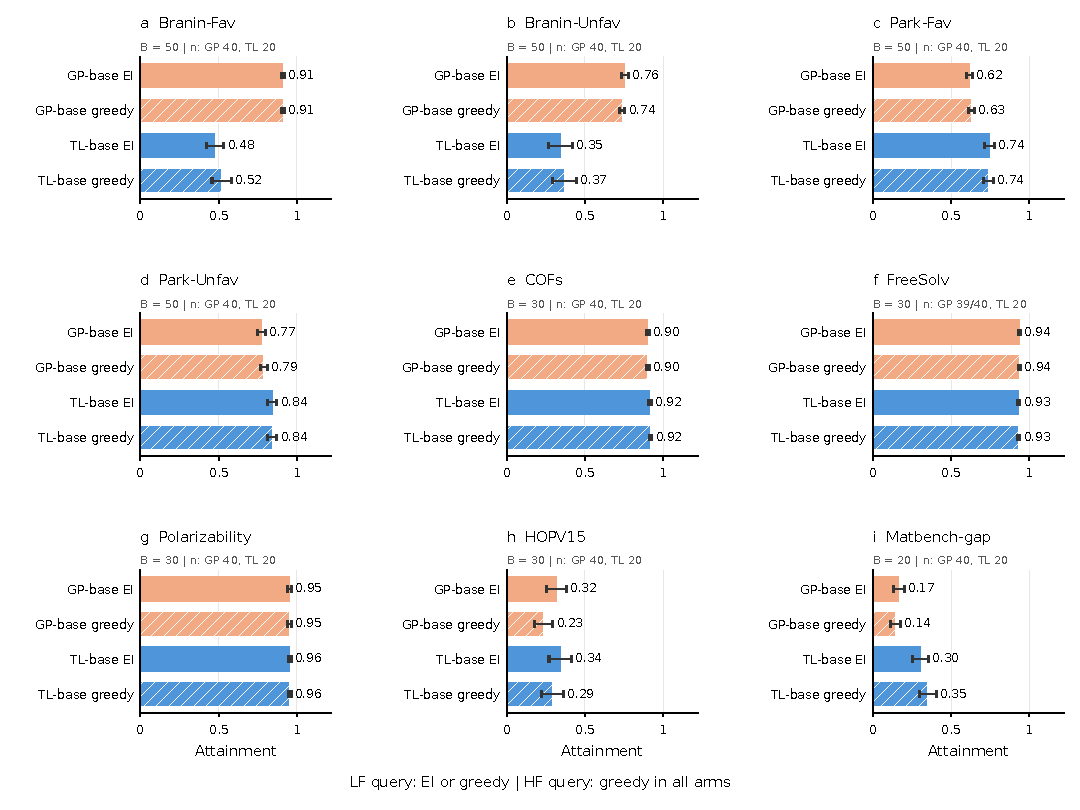
\includegraphics[width=\textwidth]{paper_figures/supp_acq_matrix.pdf}
\caption{Matched-acquisition comparison for GP-base and TL-base. \textbf{a--i,} Attainment under expected improvement (EI, solid bars) and greedy selection (hatched bars) for LF queries. HF queries use greedy selection in every arm. Orange denotes GP-base and blue denotes TL-base. Attainment follows Fig.~1, averaging the share of the budget window spent at or below the pool's top 5, 2, 1 and 0.5\% targets. Bars show mean $\pm$ s.e.\ over 40 seeds (42--81) for GP-base (39 for FreeSolv under EI) and 20 seeds (42--61) for TL-base, using the same seed set for both policies within each surrogate. Budgets match Fig.~1, except Matbench-gap at 20. TL-base values use the same runs as the EI and greedy arms in Supplementary Fig.~\ref{suppfig:portfolio}.}
\label{suppfig:acquisition}
\end{figure*}

\begin{figure*}[t]
\centering
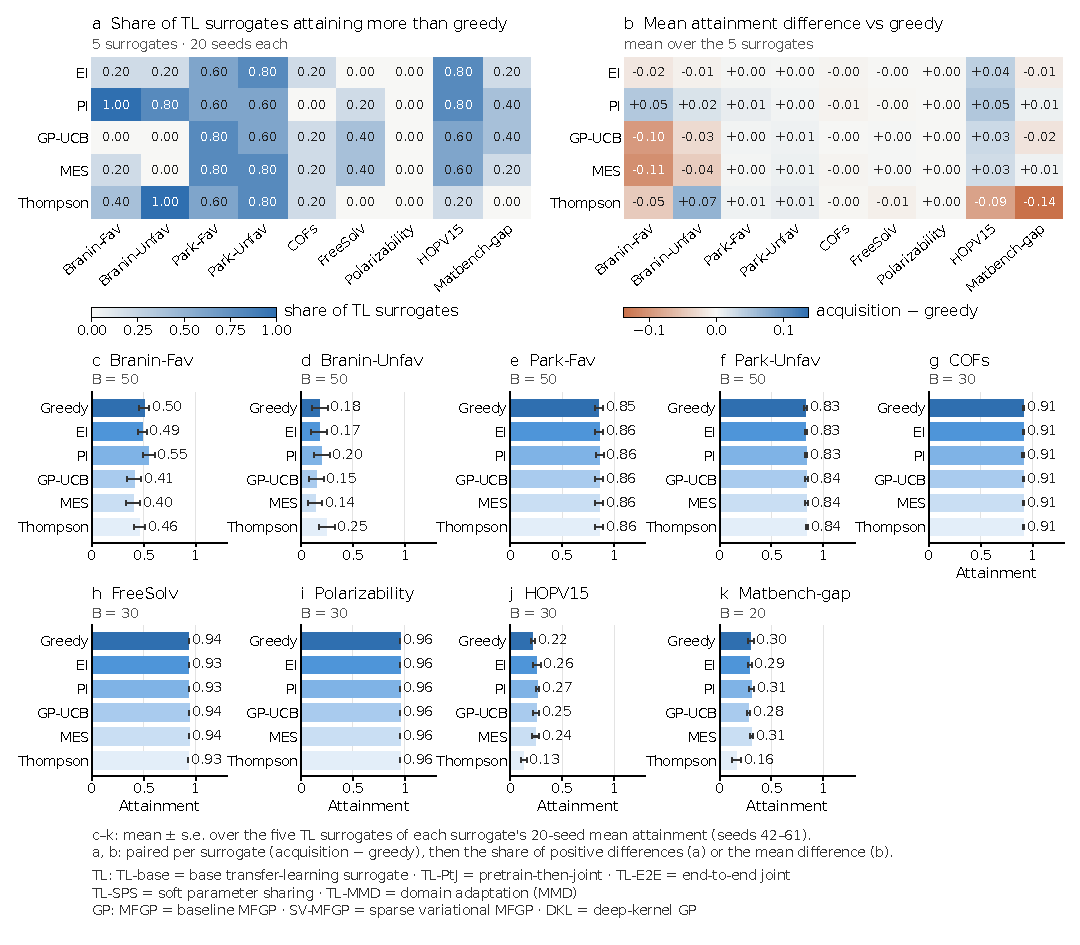
\includegraphics[width=\textwidth]{paper_figures/supp_acq_portfolio.pdf}
\caption{Acquisition portfolio under attainment. \textbf{a,} Share of the five TL surrogates whose uncertainty-driven acquisition attains more than the greedy policy on each benchmark. The acquisitions are EI, probability of improvement, the GP lower confidence bound, max-value entropy search and Thompson sampling. Each uses the BLR predictive standard deviation. \textbf{b,} Mean paired attainment difference (acquisition minus greedy) over the five surrogates. \textbf{c--k,} Attainment per acquisition, shown as mean $\pm$ s.e.\ over the five surrogates. Each surrogate value is a mean over 20 seeds (42--61). Budgets match Fig.~1, except Matbench-gap at 20.}
\label{suppfig:portfolio}
\end{figure*}


\paragraph{Calibration.} The calibration analysis of Methods~4.2 relates the loop-mean held-out LF expected calibration error (ECE) of every surrogate to its attainment from Fig.~1 (Supplementary Fig.~\ref{suppfig:calibration}a--m). Across eight surrogates and thirteen benchmarks, the correlation between loop-mean held-out LF calibration error and attainment had no consistent sign. It exceeded $|r| = 0.5$ only on Matbench-gap and ExptGap-PBE ($r = -0.67$ and $-0.90$). There, the three GPs were both the worst-calibrated LF models and the weakest optimizers. Their calibration errors spanned $0.15$--$0.36$, compared with $0.08$--$0.12$ for TL surrogates. On COFs, every surrogate attained $0.90$--$0.93$, so the small range limits interpretation of the correlation ($r = -0.48$).

Good calibration also did not identify the best optimizers. GP-base had the lowest LF calibration error on seven of thirteen benchmarks. Yet it ranked in the lower half of the eight surrogates by attainment on seven of nine molecular and materials pools. GP-DKL was the worst-calibrated on eight benchmarks but among the best optimizers on the Branin functions. ECE is averaged over refits recorded in each source run, whose horizon can differ from the attainment budget. The held-out LF calibration error uses 34--40 seeds per cell. Of 104 cells, 11 have fewer than 40. These are GP-SV on Branin-Fav and Branin-Unfav, GP-base on FreeSolv, and GP-base and GP-DKL on the four larger materials pools. For these larger pools, not every run recorded calibration error. For TL surrogates, calibration assesses the separate LF BLR head rather than the HF head driving acquisition.

\begin{figure*}[t]
\centering
%% Formerly main-text Fig. 4; moved to the SI on 2026-09-17 (letters a--m baked in).
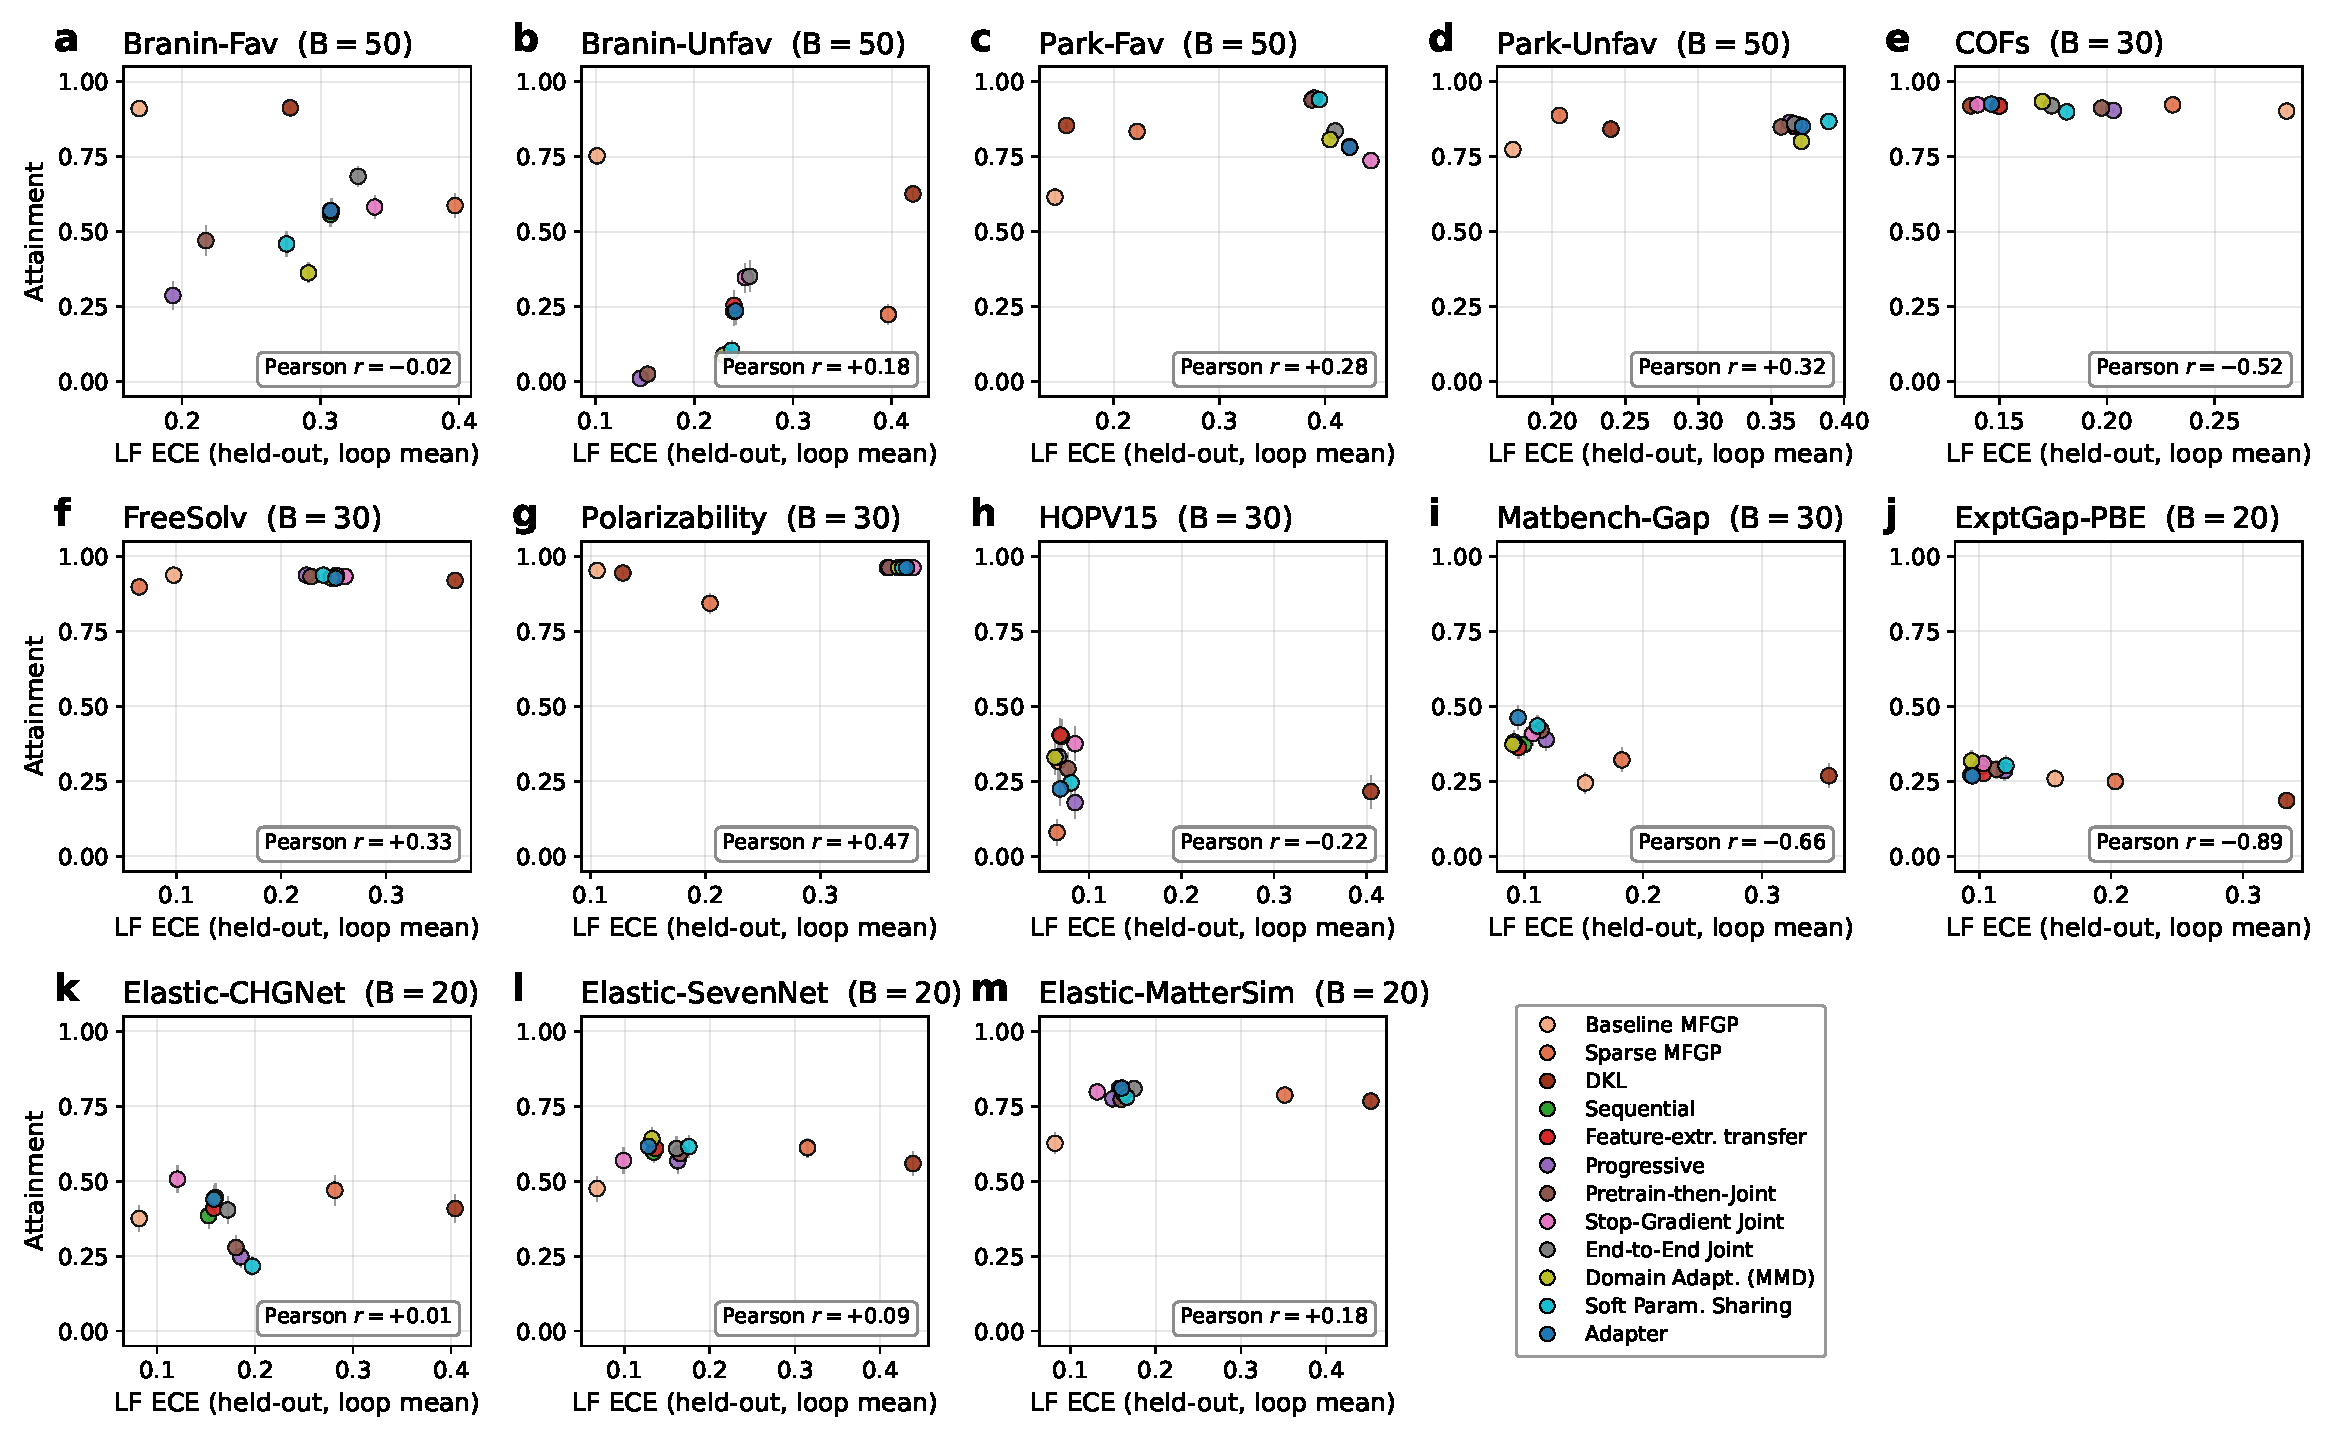
\includegraphics[width=\textwidth]{paper_figures/fig4_calibration_attain.pdf}
\caption{Calibration does not predict optimization performance.
\textbf{a--m,} Calibration versus attainment, with one panel per benchmark and one point per surrogate. Colour denotes family (orange for GPs, blue for TL), and marker denotes surrogate (legend). The horizontal axis shows held-out LF expected calibration error averaged over refits of the source runs. The vertical axis shows attainment from Fig.~1 at the displayed budget. Values are mean $\pm$ s.e.\ over 40 seeds, except 36 and 39 for GP-SV on Branin-Fav and Branin-Unfav. Each panel gives the Pearson correlation $r$ across the eight surrogate means. Because higher attainment is better, a negative $r$ associates lower calibration error with better optimization. No consistent relation appears. Only Matbench-gap and ExptGap-PBE (\textbf{i},\textbf{j}) have $|r| \ge 0.5$, and their three GP surrogates are both the worst-calibrated and least effective. On COFs, FreeSolv and Polarizability (\textbf{e}--\textbf{g}), every surrogate attains $0.84$--$0.96$. This small attainment range limits interpretation of the correlation.}
\label{suppfig:calibration}
\end{figure*}






\suppnote{Feature ablation, HF-only controls and pick logs}{suppnote:controls}

\paragraph{Feature and head-path ablations.} Supplementary Tables~\ref{supptab:feature_ablation} and~\ref{supptab:head_path} report the ablations of Methods~4.8. The head-path ablation used TL-base, whose LF prediction enters the head both as the additive offset of $\mu^{(H)}$ and as a regression column, and removed each entry point in turn with learned and with random features. Because the HF-only network has no LF network, it is listed once.

\paragraph{HF-only controls.} Supplementary Table~\ref{supptab:hf_only_baselines} compares the multi-fidelity surrogates of Fig.~1 with the two HF-only controls of Methods~4.8, a single-fidelity GP (SFGP) with EI and uniformly random HF sampling, each arm scored over its own window (definitions in the table footnotes).

\paragraph{TL-base against the GPs.} Supplementary Table~\ref{supptab:tlbase_vs_gp} lists, for every benchmark, the attainment of TL-base next to that of GP-base and of the best-performing GP on that benchmark, with the differences quoted in the main text.

\paragraph{Summary of Fig.~1o,p.} Supplementary Table~\ref{supptab:fig1_summary} lists each surrogate's mean attainment and mean deficit to the best surrogate, averaged over the thirteen benchmarks and over the nine molecular and materials benchmarks.

\paragraph{Pick logs.} Supplementary Table~\ref{supptab:hopv15_picklog} summarizes the HF pick logs of the HOPV15 runs in Fig.~2h, using the four statistics defined in Methods~4.8 and mean final regret.

\begin{table}[p]
\centering
\scriptsize
\caption{Feature ablation of the five TL surrogates on nine molecular and materials pools. Values are mean attainment over 40 seeds at $B = 30$, using the targets and window of Fig.~1. `Learned' is the reported surrogate. `Random features' replaces the head's 64-dimensional representation with features from an untrained network of the same architecture, retaining the scalar LF prediction. The `Scalar head' uses only that scalar prediction. The `HF-only network' uses the same architecture, training cost, head and initial HF points, but fits HF observations alone. It spends the whole budget on HF evaluations and contains no LF network, so it is listed once (--, not applicable).}
\label{supptab:feature_ablation}
\begin{tabular}{@{}lcccc@{}}
\toprule
Pool & Learned & Random features & Scalar head & HF-only network \\
\midrule
\multicolumn{5}{@{}l}{\emph{TL-base}} \\
COFs & 0.92 & 0.92 & 0.92 & 0.72 \\
FreeSolv & 0.93 & 0.93 & 0.93 & 0.77 \\
Polarizability & 0.96 & 0.96 & 0.96 & 0.92 \\
HOPV15 & 0.38 & 0.40 & 0.34 & 0.32 \\
Matbench-gap & 0.41 & 0.35 & 0.44 & 0.17 \\
ExptGap-PBE & 0.41 & 0.38 & 0.36 & 0.32 \\
Elastic-CHGNet & 0.62 & 0.60 & 0.50 & 0.39 \\
Elastic-SevenNet & 0.69 & 0.74 & 0.68 & 0.41 \\
Elastic-MatterSim & 0.87 & 0.88 & 0.88 & 0.39 \\
\addlinespace
\multicolumn{5}{@{}l}{\emph{TL-PtJ}} \\
COFs & 0.91 & 0.91 & 0.91 & -- \\
FreeSolv & 0.93 & 0.93 & 0.93 & -- \\
Polarizability & 0.96 & 0.96 & 0.96 & -- \\
HOPV15 & 0.29 & 0.26 & 0.22 & -- \\
Matbench-gap & 0.42 & 0.40 & 0.39 & -- \\
ExptGap-PBE & 0.38 & 0.40 & 0.35 & -- \\
Elastic-CHGNet & 0.38 & 0.35 & 0.42 & -- \\
Elastic-SevenNet & 0.70 & 0.70 & 0.67 & -- \\
Elastic-MatterSim & 0.85 & 0.86 & 0.85 & -- \\
\addlinespace
\multicolumn{5}{@{}l}{\emph{TL-E2E}} \\
COFs & 0.92 & 0.92 & 0.92 & -- \\
FreeSolv & 0.94 & 0.93 & 0.93 & -- \\
Polarizability & 0.96 & 0.96 & 0.96 & -- \\
HOPV15 & 0.33 & 0.41 & 0.38 & -- \\
Matbench-gap & 0.38 & 0.37 & 0.40 & -- \\
ExptGap-PBE & 0.36 & 0.39 & 0.41 & -- \\
Elastic-CHGNet & 0.51 & 0.52 & 0.54 & -- \\
Elastic-SevenNet & 0.73 & 0.75 & 0.71 & -- \\
Elastic-MatterSim & 0.88 & 0.88 & 0.88 & -- \\
\addlinespace
\multicolumn{5}{@{}l}{\emph{TL-SPS}} \\
COFs & 0.90 & 0.90 & 0.90 & -- \\
FreeSolv & 0.94 & 0.94 & 0.94 & -- \\
Polarizability & 0.96 & 0.96 & 0.96 & -- \\
HOPV15 & 0.25 & 0.26 & 0.16 & -- \\
Matbench-gap & 0.43 & 0.45 & 0.39 & -- \\
ExptGap-PBE & 0.41 & 0.41 & 0.47 & -- \\
Elastic-CHGNet & 0.33 & 0.34 & 0.32 & -- \\
Elastic-SevenNet & 0.73 & 0.73 & 0.67 & -- \\
Elastic-MatterSim & 0.86 & 0.85 & 0.86 & -- \\
\addlinespace
\multicolumn{5}{@{}l}{\emph{TL-MMD}} \\
COFs & 0.93 & 0.94 & 0.93 & -- \\
FreeSolv & 0.93 & 0.93 & 0.92 & -- \\
Polarizability & 0.96 & 0.96 & 0.96 & -- \\
HOPV15 & 0.33 & 0.36 & 0.39 & -- \\
Matbench-gap & 0.37 & 0.42 & 0.42 & -- \\
ExptGap-PBE & 0.40 & 0.36 & 0.41 & -- \\
Elastic-CHGNet & 0.55 & 0.51 & 0.58 & -- \\
Elastic-SevenNet & 0.75 & 0.75 & 0.75 & -- \\
Elastic-MatterSim & 0.87 & 0.87 & 0.87 & -- \\
\bottomrule
\end{tabular}
\end{table}

\begin{table}[p]
\centering
\scriptsize
\caption{Head-path ablation of TL-base on nine molecular and materials pools. Values are mean attainment over 40 seeds at $B = 30$, using the targets and window of Fig.~1. The head predicts $\mu^{(H)} = g^{(L)} + w^{\top}[\,g^{(L)}, \varphi^{(L)}, 1\,]$. `Offset' denotes the additive $g^{(L)}$ term, `input' denotes the $g^{(L)}$ regression column, and `removed' zeroes both. (1) Learned features, offset and input (the reported head). (2) Learned features, offset only. (3) Learned features, input only. (4) Learned features, $g^{(L)}$ removed from the head. (5) Random features from an untrained network of the same architecture, with $g^{(L)}$ as offset and input. (6) Random features, $g^{(L)}$ removed. Columns (1) and (5) are the Learned and Random-features configurations in Supplementary Table~\ref{supptab:feature_ablation}.}
\label{supptab:head_path}
\setlength{\tabcolsep}{3pt}%
\begin{tabular}{@{}lcccccc@{}}
\toprule
 & \multicolumn{4}{c}{Learned features} & \multicolumn{2}{c}{Random features} \\
\cmidrule(lr){2-5}\cmidrule(lr){6-7}
Pool & (1) offset + input & (2) offset only & (3) input only & (4) removed & (5) offset + input & (6) removed \\
\midrule
COFs & 0.92 & 0.92 & 0.90 & 0.69 & 0.92 & 0.63 \\
FreeSolv & 0.93 & 0.94 & 0.90 & 0.70 & 0.93 & 0.51 \\
Polarizability & 0.96 & 0.96 & 0.95 & 0.92 & 0.96 & 0.73 \\
HOPV15 & 0.38 & 0.38 & 0.17 & 0.14 & 0.40 & 0.16 \\
Matbench-gap & 0.41 & 0.39 & 0.26 & 0.05 & 0.35 & 0.06 \\
ExptGap-PBE & 0.41 & 0.35 & 0.28 & 0.16 & 0.38 & 0.14 \\
Elastic-CHGNet & 0.62 & 0.63 & 0.32 & 0.20 & 0.60 & 0.19 \\
Elastic-SevenNet & 0.69 & 0.68 & 0.59 & 0.21 & 0.74 & 0.24 \\
Elastic-MatterSim & 0.87 & 0.88 & 0.78 & 0.30 & 0.88 & 0.15 \\
\bottomrule
\end{tabular}
\end{table}

\begin{table}[p]
\centering
\scriptsize
\caption{HF-only controls and multi-fidelity surrogates on thirteen benchmarks (mean over 40 seeds). SFGP EI fits a single-fidelity GP (SFGP) to HF observations and selects queries by EI. Random HF selects HF queries uniformly. Both start from the same two initial HF points as the multi-fidelity runs and spend the whole budget on HF evaluations$^{b}$. GP-base and TL-base are the multi-fidelity surrogates in Fig.~1. Attainment uses each arm's own window, from the end of its initial design to $B$$^{a}$. Final regret is the best HF regret at $B$, in each pool's objective units (GPa for elastic-modulus pools). Footnote $c$ gives exact-optimum counts.}
\label{supptab:hf_only_baselines}
\setlength{\tabcolsep}{3.2pt}%
\begin{tabular}{@{}lc cccc cccc@{}}
\toprule
& & \multicolumn{4}{c}{Attainment} & \multicolumn{4}{c}{Final regret at $B$} \\
\cmidrule(lr){3-6}\cmidrule(lr){7-10}
& & \multicolumn{2}{c}{HF-only controls} & \multicolumn{2}{c}{Multi-fidelity} & \multicolumn{2}{c}{HF-only controls} & \multicolumn{2}{c}{Multi-fidelity} \\
\cmidrule(lr){3-4}\cmidrule(lr){5-6}\cmidrule(lr){7-8}\cmidrule(lr){9-10}
Pool & $B$ & SFGP EI & Random HF & GP-base & TL-base & SFGP EI & Random HF & GP-base & TL-base \\
\midrule
Branin-Fav & 50 & 0.84 & 0.39 & 0.91 & 0.59 & 0.00 & 0.97 & 0.02 & 0.13 \\
Branin-Unfav & 50 & 0.86 & 0.35 & 0.76 & 0.35 & 0.00 & 0.91 & 0.05 & 1.16 \\
Park-Fav & 10 & 0.21 & 0.09 & 0.09 & 0.24 & 1.02 & 1.39 & 0.02 & 0.00 \\
Park-Unfav & 10 & 0.32 & 0.22 & 0.31 & 0.44 & 0.45 & 0.88 & 0.02 & 0.00 \\
COFs & 30 & 0.49 & 0.46 & 0.90 & 0.92 & 5.48 & 4.24 & 0.00 & 0.00 \\
FreeSolv & 50 & 0.37 & 0.42 & 0.97 & 0.96 & 1.38 & 0.69 & 0.02 & 0.00 \\
Polarizability & 30 & 0.61 & 0.54 & 0.95 & 0.96 & 0.11 & 0.22 & 0.00 & 0.00 \\
HOPV15 & 30 & 0.25 & 0.36 & 0.32 & 0.38 & 2.37 & 2.03 & 2.31 & 1.27 \\
Matbench-gap & 30 & 0.21 & 0.29 & 0.25 & 0.41 & 0.49 & 0.16 & 0.12 & 0.12 \\
ExptGap-PBE & 30 & 0.43 & 0.24 & 0.33 & 0.41 & 0.22 & 0.20 & 0.11 & 0.08 \\
Elastic-CHGNet & 30 & 0.24 & 0.28 & 0.49 & 0.62 & 369 & 364 & 279 & 278 \\
Elastic-SevenNet & 30 & 0.19 & 0.18 & 0.57 & 0.69 & 229 & 229 & 155 & 129 \\
Elastic-MatterSim & 30 & 0.21 & 0.25 & 0.76 & 0.87 & 371 & 360 & 250 & 244 \\
\bottomrule
\end{tabular}
\par\smallskip
{\scriptsize
$^{a}$Windows: $B = 50$ on the Branin functions, $10$ on the Park functions and $30$ on the molecular and materials pools, except FreeSolv, evaluated at $50$. The Park and FreeSolv windows therefore differ from those of Fig.~1. The HF-only arms start their window at 2 HF-equivalent units (two farthest-point-sampled HF points), the multi-fidelity arms at the end of their LF-inclusive initial design (3 to 4.5 units). On Polarizability the five TL surrogates have identical attainment and final regret.
$^{b}$SFGP EI is a BoTorch \texttt{SingleTaskGP} (Mat\'{e}rn-5/2 ARD kernel, standardized targets, library defaults) refitted to all HF observations at every step, with the next HF query chosen by EI over the pool. Random HF follows the same protocol with the HF query drawn uniformly at random from the unevaluated candidates. Neither arm queries the LF source.
$^{c}$Seeds (of 40) whose regret reached exactly zero within the window: HOPV15, Random HF 5, SFGP EI 7, TL-base 25; Matbench-gap, SFGP EI 11, Random HF 4, GP-base 6, GP-SV 5, GP-DKL 9, TL-base 10, TL-PtJ 8, TL-E2E 9, TL-SPS 6, TL-MMD 1.
}
\end{table}

\begin{table}[p]
\centering
\scriptsize
\caption{TL-base against GP-base and the best-performing GP on thirteen benchmarks. Attainment follows Fig.~1, with mean $\pm$ s.e.\ over 40 seeds at the budgets of Fig.~1. GP-SV has 36 and 39 seeds on Branin-Fav and Branin-Unfav. The best-performing GP has the highest mean attainment on that pool. The difference $\Delta$ is TL-base minus the GP named in the preceding columns. Abbreviations are as in Fig.~1.}
\label{supptab:tlbase_vs_gp}
\setlength{\tabcolsep}{4pt}%
\begin{tabular}{@{}l ccc lcc@{}}
\toprule
& & & & \multicolumn{3}{c}{Best-performing GP} \\
\cmidrule(lr){5-7}
Pool & TL-base & GP-base & $\Delta$ & Surrogate & Attainment & $\Delta$ \\
\midrule
Branin-Fav & 0.586 $\pm$ 0.039 & 0.912 $\pm$ 0.008 & $-0.326$ & GP-DKL & 0.913 $\pm$ 0.007 & $-0.327$ \\
Branin-Unfav & 0.348 $\pm$ 0.049 & 0.756 $\pm$ 0.023 & $-0.408$ & GP-base & 0.756 $\pm$ 0.023 & $-0.408$ \\
Park-Fav & 0.737 $\pm$ 0.022 & 0.615 $\pm$ 0.018 & $+0.122$ & GP-DKL & 0.854 $\pm$ 0.010 & $-0.117$ \\
Park-Unfav & 0.855 $\pm$ 0.019 & 0.774 $\pm$ 0.024 & $+0.081$ & GP-SV & 0.888 $\pm$ 0.012 & $-0.032$ \\
COFs & 0.923 $\pm$ 0.006 & 0.902 $\pm$ 0.008 & $+0.021$ & GP-SV & 0.923 $\pm$ 0.006 & $0.000$ \\
FreeSolv & 0.934 $\pm$ 0.005 & 0.938 $\pm$ 0.005 & $-0.004$ & GP-base & 0.938 $\pm$ 0.005 & $-0.004$ \\
Polarizability & 0.963 $\pm$ 0.005 & 0.954 $\pm$ 0.011 & $+0.009$ & GP-base & 0.954 $\pm$ 0.011 & $+0.009$ \\
HOPV15 & 0.376 $\pm$ 0.056 & 0.317 $\pm$ 0.063 & $+0.058$ & GP-base & 0.317 $\pm$ 0.063 & $+0.058$ \\
Matbench-gap & 0.409 $\pm$ 0.039 & 0.245 $\pm$ 0.036 & $+0.164$ & GP-SV & 0.322 $\pm$ 0.040 & $+0.088$ \\
ExptGap-PBE & 0.406 $\pm$ 0.027 & 0.333 $\pm$ 0.031 & $+0.073$ & GP-SV & 0.337 $\pm$ 0.028 & $+0.068$ \\
Elastic-CHGNet & 0.622 $\pm$ 0.041 & 0.493 $\pm$ 0.044 & $+0.129$ & GP-DKL & 0.604 $\pm$ 0.042 & $+0.018$ \\
Elastic-SevenNet & 0.691 $\pm$ 0.037 & 0.568 $\pm$ 0.039 & $+0.123$ & GP-SV & 0.725 $\pm$ 0.030 & $-0.034$ \\
Elastic-MatterSim & 0.872 $\pm$ 0.011 & 0.757 $\pm$ 0.025 & $+0.115$ & GP-SV & 0.863 $\pm$ 0.009 & $+0.009$ \\
\bottomrule
\end{tabular}
\end{table}

\begin{table}[p]
\centering
\scriptsize
\caption{Summary of Fig.~1o,p. The table gives each surrogate's mean attainment and mean deficit to the best surrogate on each benchmark. Deficit is the benchmark's highest mean attainment minus the surrogate's mean attainment. Values are mean $\pm$ s.e.\ over benchmarks. Lower deficits are better, and 0 denotes the best attainment on every benchmark. Summaries cover all thirteen benchmarks (Fig.~1o) and the nine molecular and materials benchmarks (Fig.~1p). Surrogates are sorted by the nine-benchmark deficit. Abbreviations are as in Fig.~1.}
\label{supptab:fig1_summary}
\begin{tabular}{@{}l cc cc@{}}
\toprule
& \multicolumn{2}{c}{Thirteen benchmarks} & \multicolumn{2}{c}{Nine molecular and materials benchmarks} \\
\cmidrule(lr){2-3}\cmidrule(lr){4-5}
Surrogate & Mean attainment & Mean deficit & Mean attainment & Mean deficit \\
\midrule
TL-base & 0.671 & 0.084 $\pm$ 0.038 & 0.688 & 0.013 $\pm$ 0.007 \\
TL-MMD & 0.629 & 0.126 $\pm$ 0.060 & 0.678 & 0.023 $\pm$ 0.009 \\
TL-E2E & 0.673 & 0.081 $\pm$ 0.032 & 0.668 & 0.033 $\pm$ 0.012 \\
TL-PtJ & 0.625 & 0.130 $\pm$ 0.061 & 0.649 & 0.053 $\pm$ 0.025 \\
TL-SPS & 0.631 & 0.124 $\pm$ 0.058 & 0.647 & 0.055 $\pm$ 0.032 \\
GP-DKL & 0.686 & 0.069 $\pm$ 0.016 & 0.631 & 0.070 $\pm$ 0.021 \\
GP-SV & 0.623 & 0.131 $\pm$ 0.044 & 0.619 & 0.083 $\pm$ 0.030 \\
GP-base & 0.659 & 0.096 $\pm$ 0.027 & 0.612 & 0.089 $\pm$ 0.024 \\
\bottomrule
\end{tabular}
\end{table}


\begin{table}[p]
\centering
\scriptsize
\caption{Pick-log summary on HOPV15, using 40 seeds and $B = 30$. Mid-budget is 15 HF-equivalent units. The LF-top-ranked candidate is ranked first by the proxy and has HF regret $3.90$. `Final at LF top' gives the share of seeds ending at that candidate's regret. `Improved after 15' gives the share whose best-so-far regret improved after mid-budget. `Reached zero' counts seeds, out of 40, reaching exactly zero regret by $B = 30$. `Promoted' gives the share of second-half HF picks already evaluated at LF$^{a}$. `Final regret' gives mean final regret at $B = 30$.}
\label{supptab:hopv15_picklog}
\begin{tabular}{@{}lccccc@{}}
\toprule
Surrogate & Final at LF top & Improved after 15 & Reached zero & Promoted & Final regret \\
\midrule
GP-base & 0.45 & 0.30 & 14/40 & 1.00 & 2.31 \\
GP-SV & 0.50 & 0.38 & 3/40 & 1.00 & 3.32 \\
GP-DKL & 0.15 & 0.47 & 8/40 & 0.84 & 2.61 \\
TL-base & 0.23 & 0.62 & 25/40 & 0.99 & 1.27 \\
TL-PtJ & 0.00 & 0.62 & 20/40 & 1.00 & 1.66 \\
TL-E2E & 0.23 & 0.75 & 27/40 & 1.00 & 1.20 \\
TL-SPS & 0.00 & 0.50 & 13/40 & 1.00 & 2.44 \\
TL-MMD & 0.15 & 0.55 & 22/40 & 1.00 & 1.47 \\
\bottomrule
\end{tabular}
\par\smallskip
{\scriptsize $^{a}$Second-half picks are the HF queries issued after 15 HF-equivalent units. A pick is promoted when its candidate had already been queried at LF earlier in the same run.}
\end{table}

\suppnote{Surrogate-free LF screen and screening regimes}{suppnote:screen}

The surrogate-free screen and its screening regret are defined in Methods~4.6, which also fixes the boundary between Regime~A and Regime~B at a screening regret of $0.3$. Here we place each benchmark (Fig.~4a,b).

In Regime~A, represented by Park-Fav and Polarizability, LF--HF top-1\% overlap is approximately $1$ and screening regret is at most $0.09$. The screen therefore already identifies a near-optimal candidate. In Regime~B, high global correlation can conceal poor agreement among top-ranked candidates. COFs has a Spearman rank correlation of $0.998$ but screening regret $4.52$. Although both COFs and Polarizability have $R^2 \approx 0.96$ or higher, their screening outcomes differ. HOPV15 and Matbench-gap fall in Regime~B, with screening regrets of $3.90$ and $0.91$.

The four larger materials pools also fall in Regime~B. On ExptGap-PBE, the screen misses the optimum by $1.15$~eV. The first indexed HF optimum sits at LF rank $1{,}033$ of $3{,}508$. On the elastic-modulus pools, screening regrets are $384$~GPa for Elastic-CHGNet and $369$~GPa for Elastic-SevenNet, or $74\%$ and $97\%$ of their HF ranges. Elastic-MatterSim has screening regret $3$~GPa, or $0.6\%$ of the range, with the HF optimum at LF rank 2. These related pools therefore span nearly sufficient to uninformative screening. The best TL surrogates reached similarly low regret where screening was near-optimal and improved on it where LF rankings were less useful. On COFs, every surrogate reached zero regret within the budget (Fig.~2e).

\suppnote{Computational cost: absolute FLOPs and compute ranking}{suppnote:computational_cost}

Fig.~5 shows how surrogate compute scales with problem size. Here we report the absolute loop-integrated costs in floating-point operations (FLOPs) underlying those laws, profiled as described in Methods~4.9. GP-SV and GP-DKL required up to $22$-fold and $15$-fold the cheapest TL surrogate, respectively, and GP-base up to $5.6$-fold. GP-base was the cheapest surrogate on Park-Unfav, Polarizability and HOPV15. TL-PtJ was the cheapest TL surrogate on every benchmark. Average compute ranks across the nine benchmarks, where lower is cheaper, are $1.3$ for TL-PtJ, $2.3$ for TL-SPS and $3.3$ for TL-MMD. TL-base and GP-base both rank $4.3$, followed by TL-E2E at $5.3$, GP-DKL at $7.0$ and GP-SV at $8.0$.

\begin{figure*}[t]
\centering
%%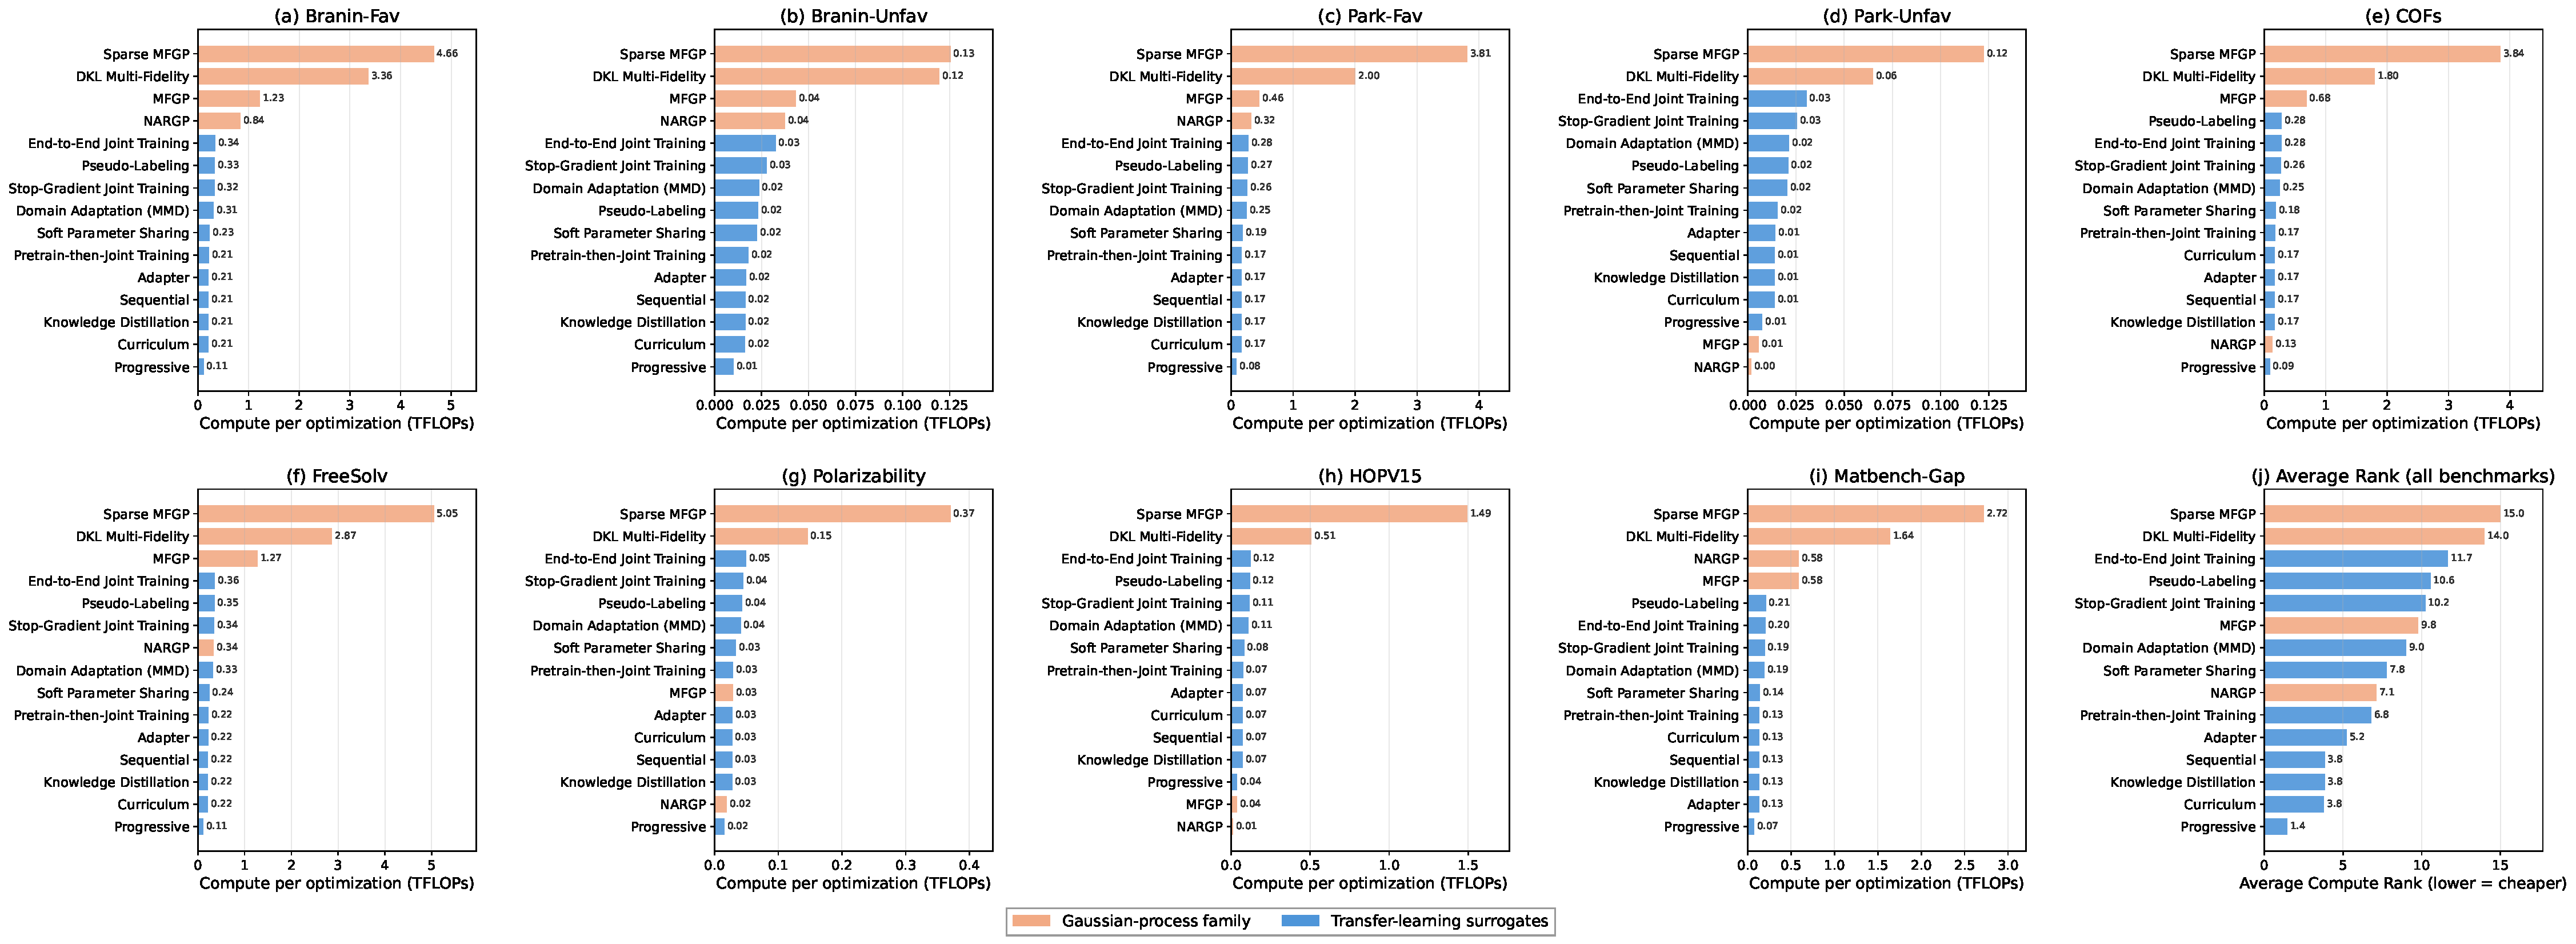
\includegraphics[width=\textwidth]{paper_figures/computing_time.pdf}
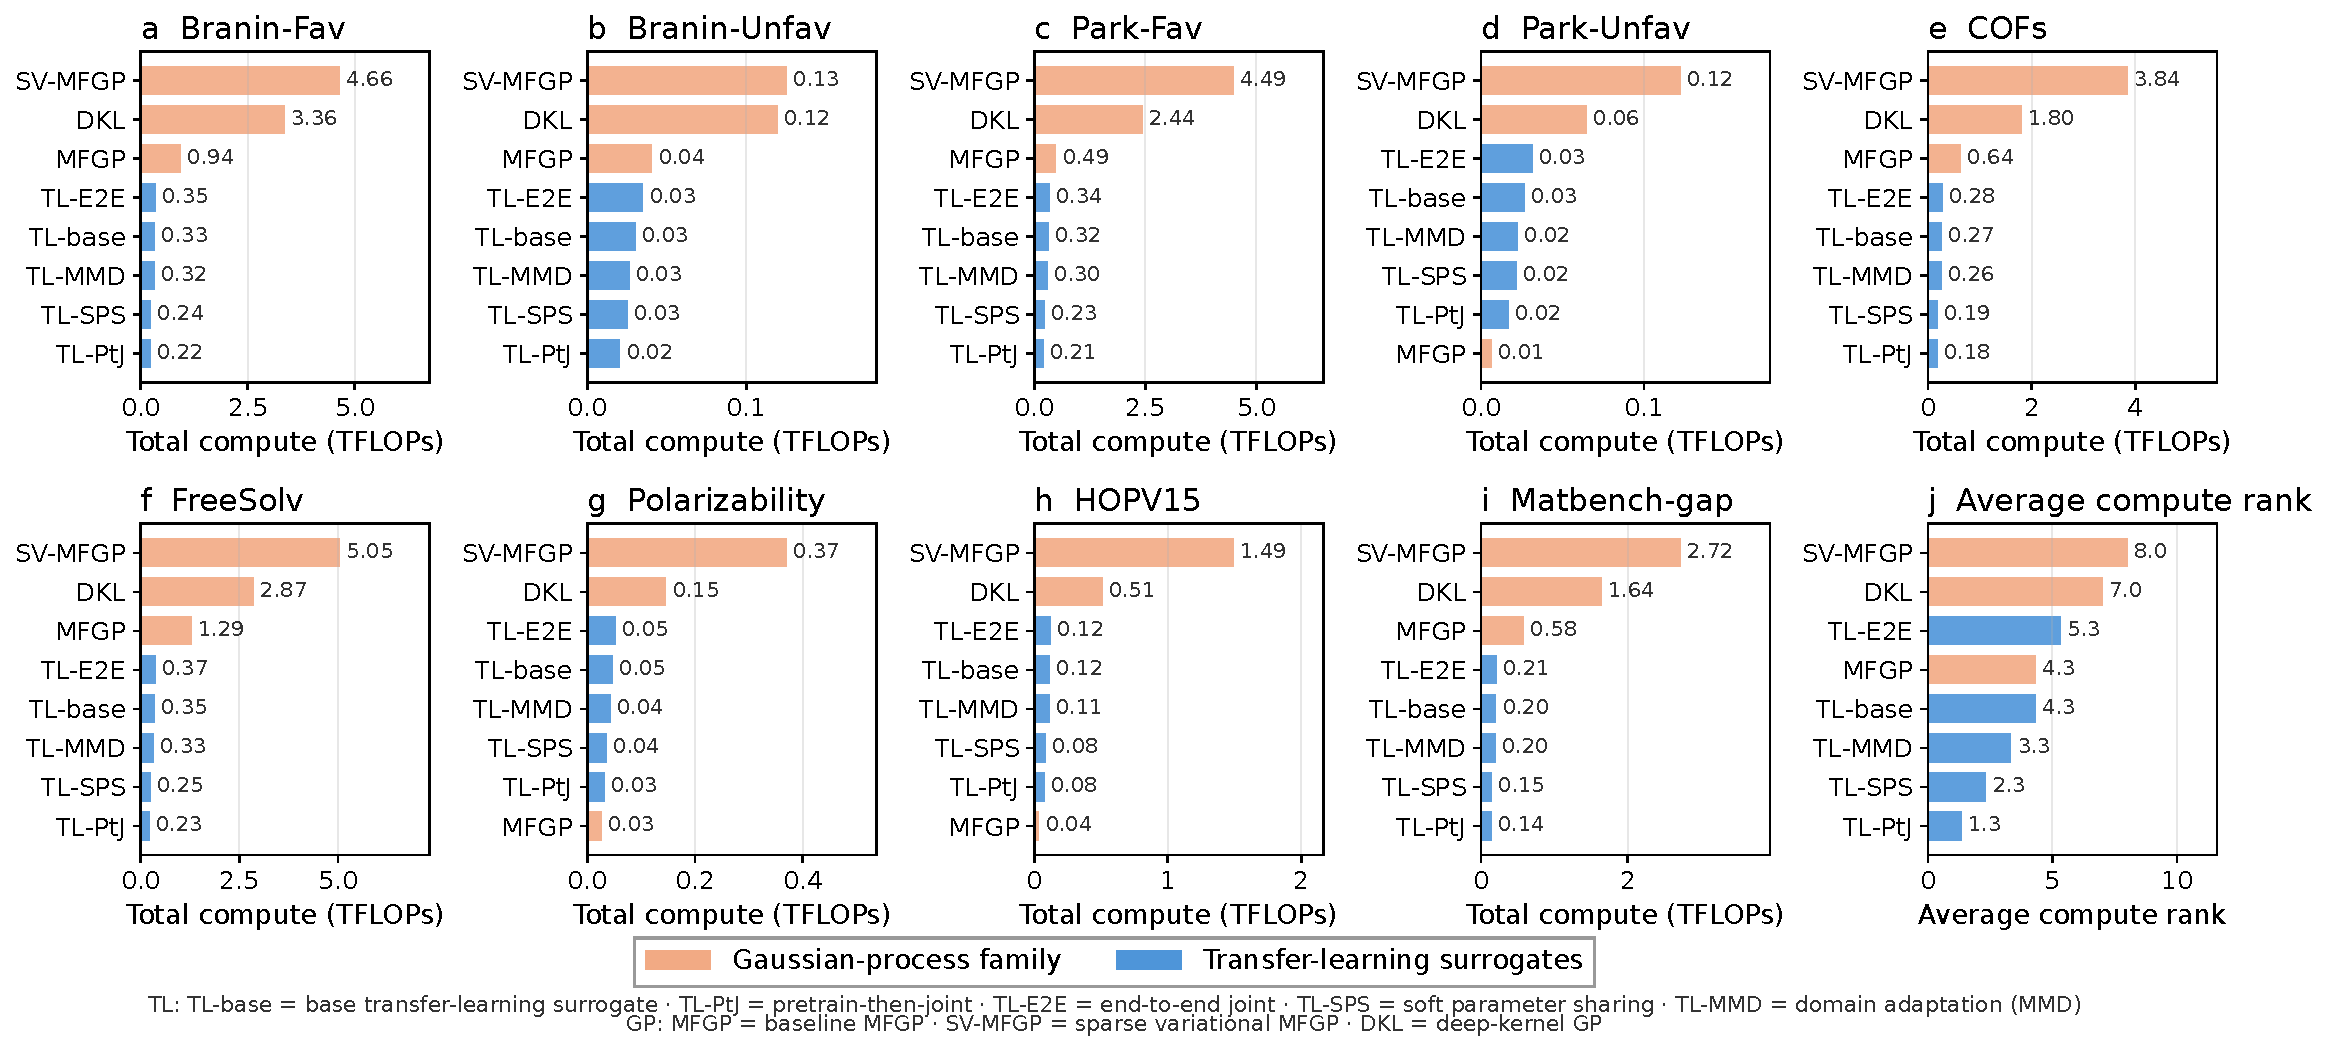
\includegraphics[width=\textwidth]{paper_figures/computing_time_blr.pdf}
\caption{Absolute computational cost across nine of the thirteen benchmarks. Hardware-independent floating-point operations (FLOPs) cover one surrogate fit and one pool-wide prediction per iteration. Costs are interpolated from profiled training-set sizes and summed over the MFBO loop. Orange denotes the GP family, and blue denotes TL surrogates. GP-SV and GP-DKL are the most expensive on every benchmark, costing up to roughly $22$-fold and $15$-fold the cheapest TL surrogate, respectively. GP-base scales as $\mathcal{O}(N^3)$ in observation count, with measured fit-FLOP exponent $k = 3.0$. TL surrogates scale as $\mathcal{O}(N)$, with $k = 0.9$--$1.0$, so the gap widens with budget. Panel \textbf{j} summarizes average compute rank across nine benchmarks, with lower values indicating lower cost. A shared legend below the panels repeats the family colours. Profiles cover all five TL surrogates and the three-member GP family, including the BLR head and residual network. Abbreviations are as in Fig.~1. FLOPs are accumulated over the budgets of Fig.~1, except FreeSolv at 50 and Matbench-gap at 20. GP-base is the cheapest surrogate on Park-Unfav, Polarizability and HOPV15.}
\label{suppfig:computing_time}
\end{figure*}



\fi

\end{document}
